\flushbottom


%% add sections to exercises


%%=============================================================================
%%=============================================================================
\chapter{Techniques for Linear Differential Equations}
\label{chapter_tflo}



My new goal in life is to take the meaningless drivel out of human interaction.

\begin{flushright}
  -Dave Ozenne
\end{flushright}




The $n^{\mathrm{th}}$ order linear homogeneous differential equation
can be written in the form:
\[
y^{(n)} + a_{n-1}(x) y^{(n-1)} + \cdots + a_1(x) y' + a_0(x) y = 0.
\]
In general it is not possible to solve second order and higher linear
differential equations.  In this chapter we will examine equations that have 
special forms which allow us to either reduce the order of the equation or 
solve it.





%%=============================================================================
\section{Constant Coefficient Equations}
\index{differential equations!constant coefficient}
\index{constant coefficient differential equations}


The $n^{\mathrm{th}}$ order constant coefficient differential equation
has the form:
\[
y^{(n)} + a_{n-1} y^{(n-1)} + \cdots + a_1 y' + a_0 y = 0.
\]
We will find that solving a constant coefficient differential equation is 
no more difficult than finding the roots of a polynomial.  For notational 
simplicity, we will first consider second order equations.  Then we will 
apply the same techniques to higher order equations.



%%-----------------------------------------------------------------------------
\subsection{Second Order Equations}





\paragraph{Factoring the Differential Equation.}
Consider the second order constant coefficient differential equation:
\begin{equation}
  \label{second_order_constant_coefficient}
  y'' + 2 a y' + b y = 0.
\end{equation}
Just as we can factor a second degree polynomial:
\begin{gather}
  \label{quadratic_lambda}
  \lambda^2 + 2 a \lambda + b = (\lambda - \alpha)(\lambda - \beta),
  \nonumber
  \alpha = -a + \sqrt{a^2 - b} \quad \mathrm{and} \quad
  \beta = -a - \sqrt{a^2 - b},
\end{gather}
we can factor Equation~\ref{second_order_constant_coefficient}.
\[
\left( \frac{\dd^2}{\dd x^2} + 2 a \frac{\dd}{\dd x} + b \right) y  =
\left( \frac{\dd}{\dd x} - \alpha \right) \left( \frac{\dd}{\dd x} - \beta \right) y
\]
Once we have factored the differential equation, we can solve it by 
solving a series of two first order differential equations.
We set $u = \left( \frac{\dd}{\dd x} - \beta \right) y$ to obtain a first order
equation:
\[
\left( \frac{\dd}{\dd x} - \alpha \right) u = 0,
\]
which has the solution:
\[
u = c_1 \e^{\alpha x}.
\]
To find the solution of Equation~\ref{second_order_constant_coefficient},
we solve
\[
\left( \frac{\dd}{\dd x} - \beta \right) y = u = c_1 \e^{\alpha x}.
\]
We multiply by the integrating factor and integrate.
\begin{gather*}
  \frac{\dd}{\dd x} \left( \e^{-\beta x} y \right) = c_1 \e^{(\alpha - \beta) x} 
  \\
  y = c_1 \e^{\beta x} \int \e^{(\alpha - \beta) x} \,\dd x + c_2 \e^{\beta x}
\end{gather*}
We first consider the case that $\alpha$ and $\beta$ are distinct.
\[
y = c_1 \e^{\beta x} \frac{1}{\alpha - \beta} \e^{(\alpha - \beta) x} + c_2 \e^{\beta x}
\]
We choose new constants to write the solution in a simpler form.
\[
y = c_1 \e^{\alpha x} + c_2 \e^{\beta x}
\]
Now we consider the case $\alpha = \beta$.
\begin{gather*}
  y = c_1 \e^{\alpha x} \int 1 \,\dd x + c_2 \e^{\alpha x} 
  \\
  y = c_1 x \e^{\alpha x} + c_2 \e^{\alpha x}
\end{gather*}
The solution of Equation~\ref{second_order_constant_coefficient} is
\begin{equation}
  \label{equation solution 2nd order const coeff factor}
  y = \begin{cases}
    c_1 \e^{\alpha x} + c_2 \e^{\beta x}, &\alpha \neq \beta, \\
    c_1 \e^{\alpha x} + c_2 x \e^{\alpha x}, &\alpha = \beta.
  \end{cases}
\end{equation}






\begin{Example}
  Consider the differential equation: $y'' + y = 0$.  
  To obtain the general solution, we factor the equation and apply the 
  result in Equation~\ref{equation solution 2nd order const coeff factor}.
  \begin{gather*}
    \left( \frac{\dd}{\dd x} - \imath \right) 
    \left( \frac{\dd}{\dd x} + \imath \right) y = 0
    \\
    y = c_1 \e^{\imath x} + c_2 \e^{-\imath x}.
  \end{gather*}
\end{Example}







\begin{Example}
  Next we solve $y'' = 0$.
  \begin{gather*}
    \left( \frac{\dd}{\dd x} - 0 \right) 
    \left( \frac{\dd}{\dd x} - 0 \right) y = 0
    \\
    y = c_1 \e^{0 x} + c_2 x \e^{0 x} 
    \\
    y = c_1 + c_2 x
  \end{gather*}
\end{Example}






\paragraph{Substituting the Form of the Solution into the Differential 
  Equation.}
Note that if we substitute $y = \e^{\lambda x}$ into the differential 
equation (\ref{second_order_constant_coefficient}), we will obtain the 
quadratic polynomial (\ref{quadratic_lambda}) for $\lambda$.
\begin{gather*}
  y'' + 2 a y' + b y = 0 
  \\
  \lambda^2 \e^{\lambda x} + 2 a \lambda \e^{\lambda x} + b \e^{\lambda x} = 0 
  \\
  \lambda^2 + 2 a \lambda + b = 0
\end{gather*}
This gives us a superficially different method for solving constant 
coefficient equations.
We substitute $y = \e^{\lambda x}$ into the differential equation.
Let $\alpha$ and $\beta$ be the roots of the quadratic in $\lambda$.  If
the roots are distinct, then the linearly independent solutions are
$y_1 = \e^{\alpha x}$ and $y_2 = \e^{\beta x}$.  If the quadratic has 
a double root at $\lambda = \alpha$, then the linearly independent solutions
are $y_1 = \e^{\alpha x}$ and $y_2 = x \e^{\alpha x}$.




\begin{Example}
  Consider the equation:
  \[ 
  y'' - 3 y' + 2y = 0.
  \]
  The substitution $y = \e^{\lambda x}$ yields
  \[
  \lambda^2 - 3 \lambda + 2 = (\lambda-1)(\lambda-2) = 0.
  \]
  Thus the solutions are $\e^x$ and $\e^{2x}$.
\end{Example}






\begin{Example}
  Next consider the equation:
  \[ 
  y'' - 2 y' + 4 y = 0.
  \]
  The substitution $y = \e^{\lambda x}$ yields
  \[
  \lambda^2 - 2 \lambda + 4 = (\lambda-2)^2 = 0.
  \]
  Because the polynomial has a double root, the solutions are 
  $\e^{2x}$ and $x \e^{2x}$.
\end{Example}







\begin{Result}
  \label{second order constant coefficient factor}
  Consider the second order constant coefficient differential equation:
  \[
  y'' + 2 a y' + b y = 0.
  \]
  We can factor the differential equation into the form:
  \[
  \left( \frac{\dd}{\dd x} - \alpha \right) 
  \left( \frac{\dd}{\dd x} - \beta \right) y = 0,
  \]
  which has the solution:
  \[
  y = \begin{cases}
    c_1 \e^{\alpha x} + c_2 \e^{\beta x}, &\alpha \neq \beta, \\
    c_1 \e^{\alpha x} + c_2 x \e^{\alpha x}, &\alpha = \beta.
  \end{cases}
  \]
  We can also determine $\alpha$ and $\beta$ by substituting $y = \e^{\lambda x}$ into the 
  differential equation and factoring the polynomial in $\lambda$.
\end{Result}




%% CONTINUE: Talk about initial conditions.




\paragraph{Shift Invariance.}
Note that if $u(x)$ is a solution of a constant coefficient equation,
then $u(x+c)$ is also a solution.  This is useful in applying 
initial or boundary conditions.




\begin{Example}
  Consider the problem
  \[ 
  y'' - 3 y' + 2 y = 0, \qquad y(0) = a, \quad y'(0) = b.
  \]
  We know that the general solution is
  \[
  y = c_1 \e^x + c_2 \e^{2x}.
  \]
  Applying the initial conditions, we obtain the equations,
  \[
  c_1 + c_2 = a, \quad c_1 + 2 c_2 = b.
  \]
  The solution is
  \[
  y = (2 a - b) \e^x + (b - a) \e^{2 x}.
  \]
  Now suppose we wish to solve the same differential equation with the 
  boundary conditions $y(1) = a$ and $y'(1) = b$.  All we have to do is 
  shift the solution to the right.
  \[
  y = (2 a - b) \e^{x-1} + (b - a) \e^{2 (x-1)}.
  \]
\end{Example}











%%-----------------------------------------------------------------------------
\subsection{Real-Valued Solutions}




If the coefficients of the differential equation are real, then the solution
can be written in terms of real-valued functions
(Result~\ref{result nth order linear ode, nature of solutions}).   
For a real root $\lambda = \alpha$ of the polynomial in $\lambda$, the corresponding
solution, $y = \e^{\alpha x}$, is real-valued.  

Now recall that the complex
roots of a polynomial with real coefficients occur in complex conjugate
pairs.  Assume that $\alpha \pm \imath \beta$ are roots of
\[
\lambda^n + a_{n-1} \lambda^{n-1} + \cdots + a_1 \lambda + a_0 = 0.
\]
The corresponding solutions of the differential equation are
$\e^{(\alpha + \imath \beta)x}$ and $\e^{(\alpha - \imath \beta)x}$.  Note that the
linear combinations
\[
\frac{ \e^{(\alpha + \imath \beta)x} + \e^{(\alpha - \imath \beta)x}}{2}
= \e^{\alpha x} \cos (\beta x), \qquad
\frac{ \e^{(\alpha + \imath \beta)x} - \e^{(\alpha - \imath \beta)x}}{\imath 2}
= \e^{\alpha x} \sin (\beta x),
\]
are real-valued solutions of the differential equation.
We could also obtain real-valued solution by taking the real and imaginary
parts of either $\e^{(\alpha + \imath \beta)x}$ or $\e^{(\alpha - \imath \beta)x}$.  
\[
\Re \left( \e^{(\alpha + \imath \beta)x} \right) = \e^{\alpha x} \cos(\beta x), \qquad
\Im \left( \e^{(\alpha + \imath \beta)x} \right) = \e^{\alpha x} \sin(\beta x)
\]





\begin{Example}
  Consider the equation
  \[ 
  y'' - 2 y' + 2 y = 0.
  \]
  The substitution $y = \e^{\lambda x}$ yields
  \[ 
  \lambda^2 - 2 \lambda + 2 = (\lambda -1 -\imath)(\lambda -1 + \imath) = 0. 
  \]
  The linearly independent solutions are
  \[ 
  \e^{(1 + \imath)x}, \quad \mathrm{and} \quad \e^{(1 - \imath)x}.
  \]
  We can write the general solution in terms of real functions.
  \[ 
  \boxed{
    y = c_1 \e^x \cos x + c_2 \e^x \sin x
    } 
  \]
\end{Example}




%% Find the general solution of y'' + 2 a y' + b y = 0
\begin{Exercise}
  \label{exercise y+2ay+by}
  \label{gen_soln_const_coeff}
  Find the general solution of
  \[
  y'' + 2 a y' + b y = 0
  \]
  for $a,b \in \mathbb{R}$.  There are three distinct forms of the solution
  depending on the sign of $a^2 - b$.

  \hintsolution{y+2ay+by}
\end{Exercise}



%% Find the fundamental set of solutions of y'' + 2 a y' + b y = 0
\begin{Exercise}
  \label{exercise fund set y+2ay+by}
  %% CONTINUE remove this one.
  \label{fund_set_const_coeff}
  Find the 
  \hyperref[section The Fundamental Set of Solutions]
    {fundamental set of solutions}
  of
  \[
  y'' + 2 a y' + b y = 0
  \]
  at the point $x = 0$, for $a,b \in \mathbb{R}$.  
  Use the general solutions obtained in Exercise~\ref{gen_soln_const_coeff}.

  \hintsolution{fund set y+2ay+by}
\end{Exercise}





\begin{Result}
  \label{const_coeff_diff_eqn}.
  Consider the second order constant coefficient equation
  \[
  y'' + 2 a y' + b y = 0.
  \]
  The general solution of this differential equation is
  \[
  y = 
  \begin{cases}
    \e^{-a x} \left( c_1 \e^{\sqrt{a^2-b}\,x} 
      + c_2 \e^{-\sqrt{a^2-b}\,x} \right)
    \quad &\mathrm{if}\ a^2 > b, \\
    \e^{-a x} \left( c_1 \cos (\sqrt{b - a^2}\,x) 
      + c_2 \sin(\sqrt{b-a^2}\,x) \right)
    \quad &\mathrm{if}\ a^2 < b, \\
    \e^{-a x} ( c_1 + c_2 x ) 
    \quad &\mathrm{if}\ a^2 = b. 
  \end{cases}
  \]
  The 
  \hyperref[section The Fundamental Set of Solutions]
  {fundamental set of solutions}
  at $x = 0$ is
  \begin{small}
    \[
    \begin{cases}
      \left\{
        \e^{-a x} \left( \cosh (\sqrt{a^2 - b}\, x) 
          + \frac{a}{\sqrt{a^2-b}} \sinh (\sqrt{a^2 - b}\, x) \right),
        \e^{-a x} \frac{1}{\sqrt{a^2-b}} \sinh (\sqrt{a^2 - b}\, x)
      \right\}
      \quad &\mathrm{if}\ a^2 > b, \\
      \left\{
        \e^{-a x} \left( \cos (\sqrt{b - a^2}\, x) 
          + \frac{a}{\sqrt{b - a^2}} \sin (\sqrt{b - a^2}\, x) \right),
        \e^{-a x} \frac{1}{\sqrt{b - a^2}} \sin (\sqrt{b - a^2}\, x)
      \right\}
      \quad &\mathrm{if}\ a^2 < b, \\
      \left\{
        (1 + a x) \e^{-a x},
        x \e^{-a x} 
      \right\}
      \quad &\mathrm{if}\ a^2 = b. 
    \end{cases}
    \]
  \end{small}
  To obtain the 
  \hyperref[section The Fundamental Set of Solutions]
  {fundamental set of solutions}
  at the point $x = \xi$, substitute
  $(x - \xi)$ for $x$ in the above solutions.
\end{Result}







%%-----------------------------------------------------------------------------
\subsection{Higher Order Equations}



The constant coefficient equation of order $n$ has the form
\begin{equation}
  \label{Ly=yn+an-1yn-1++a0y=0}
  L[y] = y^{(n)} + a_{n-1} y^{(n-1)} +  \cdots + a_1 y' + a_0 y = 0.
\end{equation}
The substitution $y = \e^{\lambda x}$ will transform this 
differential equation into an algebraic equation.
\begin{gather*}
  L[\e^{\lambda x} ] = \lambda^n \e^{\lambda x} 
  + a_{n-1} \lambda^{n-1} \e^{\lambda x} + \cdots 
  + a_1 \lambda \e^{\lambda x} + a_0 \e^{\lambda x} = 0 \\
  \big(\lambda^n + a_{n-1} \lambda^{n-1} + \cdots + a_1 \lambda + a_0 
  \big) \e^{\lambda x} = 0  \\
  \lambda^n + a_{n-1} \lambda^{n-1} + \cdots + a_1 \lambda + a_0 = 0 
\end{gather*}
Assume that the roots of this equation, $\lambda_1, \ldots, \lambda_n$, 
are distinct.  Then the $n$ linearly independent solutions of
Equation~\ref{Ly=yn+an-1yn-1++a0y=0} are
\[ 
\e^{\lambda_1 x}, \ldots, \e^{\lambda_n x}.
\]


If the roots of the algebraic equation are not distinct then we will not obtain
all the solutions of the differential equation.  Suppose that $\lambda_1 = \alpha$ is a 
double root.  We substitute $y = \e^{\lambda x}$ into the differential equation.
\[ 
L[\e^{\lambda x}] = [(\lambda-\alpha)^2(\lambda-\lambda_3)\cdots (\lambda-\lambda_n)] \e^{\lambda x} = 0
\]
Setting $\lambda = \alpha$ will make the left side
of the equation zero.  Thus $y = \e^{\alpha x}$ is a solution.
Now we differentiate both sides of the equation with respect to $\lambda$
and interchange the order of differentiation.
\[
\frac{\dd}{\dd \lambda} L[\e^{\lambda x}] 
= L\left[ \frac{\dd}{\dd \lambda} \e^{\lambda x} \right]
= L \left[ x \e^{\lambda x} \right]
\]
Let $p(\lambda) = (\lambda-\lambda_3)\cdots(\lambda-\lambda_n)$.  We calculate $L \left[ x \e^{\lambda x} \right]$ by
applying $L$ and then differentiating with respect to $\lambda$.
\begin{align*}
  L \left[ x \e^{\lambda x} \right]
  &= \frac{\dd}{\dd \lambda} L[\e^{\lambda x}] \\
  &= \frac{\dd}{\dd \lambda} [(\lambda-\alpha)^2(\lambda-\lambda_3)\cdots(\lambda-\lambda_n)] \e^{\lambda x} \\
  &= \frac{\dd}{\dd \lambda} [(\lambda-\alpha)^2p(\lambda)] \e^{\lambda x} \\
  &= \left[ 2(\lambda-\alpha)p(\lambda) + (\lambda-\alpha)^2 p'(\lambda) + (\lambda-\alpha)^2 p(\lambda) x \right] \e^{\lambda x} \\
  &= (\lambda - \alpha) \left[ 2p(\lambda) + (\lambda - \alpha) p'(\lambda) + (\lambda-\alpha)p(\lambda) x \right] \e^{\lambda x}
\end{align*}
Since setting $\lambda = \alpha$ will make this expression zero, $L[x \e^{\alpha x}] = 0$,
$x \e^{\alpha x}$ is a solution of Equation~\ref{Ly=yn+an-1yn-1++a0y=0}.
You can verify that $\e^{\alpha x}$ and
$x \e^{\alpha x}$ are linearly independent.  Now we have generated all of the
solutions for the differential equation.  

If $\lambda = \alpha$ is a root of multiplicity $m$ then by repeatedly 
differentiating with respect to $\lambda$ you can show that the corresponding
solutions are 
\[ 
\e^{\alpha x}, x \e^{\alpha x}, x^2 \e^{\alpha x}, \ldots, x^{m-1} \e^{\alpha x}. 
\]







\begin{Example}
  Consider the equation
  \[ 
  y''' - 3 y' + 2 y = 0. 
  \]
  The substitution $y=\e^{\lambda x}$ yields
  \[ 
  \lambda^3 - 3 \lambda + 2 = (\lambda-1)^2 (\lambda +2) = 0.
  \]
  Thus the general solution is
  \[ 
  \boxed{ 
    y = c_1 \e^x + c_2 x \e^x + c_3 \e^{-2x}.
    } 
  \]
\end{Example}











\begin{Result}
  Consider the $n^{t h}$ order constant coefficient equation
  \[ 
  \frac{\dd^n y}{\dd x^n} + a_{n-1} \frac{\dd^{n-1} y}{\dd x^{n-1}} + 
  \cdots + a_1 \frac{\dd y}{\dd x} + a_0 y = 0. 
  \]
  Let the factorization of the algebraic equation obtained with the substitution
  $y = \e^{\lambda x}$ be
  \[ 
  (\lambda-\lambda_1)^{m_1}(\lambda-\lambda_2)^{m_2} \cdots (\lambda-\lambda_p)^{m_p} = 0.
  \]
  A set of linearly independent solutions is given by
  \[ 
  \{\e^{\lambda_1 x}, x \e^{\lambda_1 x}, \ldots, x^{m_1-1} \e^{\lambda_1 x}, 
  \ldots, \e^{\lambda_p x}, x \e^{\lambda_p x}, \ldots, x^{m_p-1} \e^{\lambda_p x} \}. 
  \]
  If the coefficients of the differential equation are real, then we can 
  find a real-valued set of solutions.
\end{Result}





\begin{Example}
  Consider the equation
  \[ 
  \frac{\dd^4 y}{\dd x^4} + 2 \frac{\dd^2 y}{\dd x^2} + y = 0. 
  \]
  The substitution $y = \e^{\lambda x}$ yields
  \[ 
  \lambda^4 + 2\lambda^2 + 1 = (\lambda-i)^2(\lambda+i)^2 = 0.
  \]
  Thus the linearly independent solutions are
  \[ 
  \e^{\imath x}, x \e^{\imath x}, \e^{-\imath x}\ \mathrm{and}\ x \e^{-\imath x}. 
  \]
  Noting that 
  \[ 
  \e^{\imath x} = \cos(x) + \imath \sin(x),
  \]
  we can write the general solution in terms of sines and cosines.
  \[ 
  \boxed{ 
    y = c_1 \cos x + c_2 \sin x + c_3 x \cos x + c_4 x \sin x
    } 
  \]
\end{Example}










%%============================================================================
\section{Euler Equations}
\index{differential equations!Euler}
\index{Euler differential equations}
\index{equidimensional differential equations}




Consider the equation
\[
L[y] = x^2 \frac{\dd^2 y}{\dd x^2} + a x \frac{\dd y}{\dd x} + b y = 0, 
\quad x > 0.
\]
Let's say, for example, that $y$ has units of distance and $x$ has 
units of time.  Note that each term in the differential equation has the same 
dimension.
\[
(\mathrm{time})^2 \frac{(\mathrm{distance})}{(\mathrm{time})^2} 
= (\mathrm{time}) \frac{(\mathrm{distance})}{(\mathrm{time})}
= (\mathrm{distance}) 
\]
Thus this is a second order Euler, or equidimensional equation.
We know that the first order Euler equation, $x y' + a y = 0$, has 
the solution $y = c x^a$.  Thus for the second order equation we will
try a solution of the form $y = x^\lambda$.
The substitution $y = x^\lambda$ will transform the differential equation
into an algebraic equation.
\begin{gather*}
  L[x^\lambda] = x^2 \frac{\dd^2}{\dd x^2}[x^\lambda] + a x \frac{\dd}{\dd x} [x^\lambda] + b x^\lambda = 0\\
  \lambda(\lambda-1)x^\lambda + a \lambda x^\lambda + b x^\lambda = 0 \\
  \lambda(\lambda-1) + a \lambda + b = 0 \\
  \intertext{Factoring yields}
  (\lambda-\lambda_1)(\lambda-\lambda_2) = 0.
\end{gather*}
If the two roots, $\lambda_1$ and $\lambda_2$, are distinct then
the general solution is
\[ 
y = c_1 x^{\lambda_1} + c_2 x^{\lambda_2}. 
\]
If the roots are not distinct, $\lambda_1 = \lambda_2 = \lambda$, then we only
have the one solution, $y = x^\lambda$.  To generate the other solution we 
use the same approach as for the constant coefficient equation.  We substitute
$y = x^\lambda$ into the differential equation and differentiate with
respect to $\lambda$.
\begin{align*}
  \frac{\dd}{\dd \lambda}L[x^\lambda] 
  &= L[\frac{\dd}{\dd \lambda} x^\lambda] \\
  &= L[\ln x \ x^\lambda]
\end{align*}
Note that
\[ 
\frac{\dd}{\dd \lambda}x^\lambda = \frac{\dd}{\dd \lambda} \e^{\lambda \ln x}
= \ln x \ \e^{\lambda \ln x} = \ln x \ x^\lambda.
\]
Now we apply $L$ and then differentiate with respect to $\lambda$.
\begin{align*}
  \frac{\dd}{\dd \lambda} L[x^\lambda] 
  &= \frac{\dd}{\dd \lambda} (\lambda-\alpha)^2 x^\lambda \\
  &= 2 (\lambda-\alpha) x^\lambda + (\lambda-\alpha)^2 \ln x\ x^\lambda
\end{align*}
Equating these two results,
\[ 
L[\ln x\ x^\lambda] = 2 (\lambda-\alpha) x^\lambda + (\lambda-\alpha)^2 \ln x\ x^\lambda.
\]
Setting $\lambda = \alpha$ will make the right hand side zero.  Thus 
$y= \ln x\ x^\alpha$ is a solution.  

If you are in the mood for a little algebra you can show 
by repeatedly differentiating with respect to $\lambda$ that if 
$\lambda = \alpha$ is a root of multiplicity $m$ in an $n^{t h}$ order Euler
equation then the associated solutions are
\[ 
x^\alpha, \ln x\ x^\alpha, (\ln x)^2 x^\alpha, \ldots, (\ln x)^{m-1} x^\alpha. 
\]


\begin{Example}
  Consider the Euler equation
  \[
  x y'' - y' + \frac{y}{x} = 0.
  \]
  The substitution $y = x^\lambda$ yields the algebraic equation
  \[ 
  \lambda(\lambda-1) - \lambda + 1 = (\lambda-1)^2 = 0.
  \]
  Thus the general solution is
  \[ 
  \boxed{
    y = c_1 x + c_2 x \ln x.
    }
  \]
\end{Example}






%%-----------------------------------------------------------------------------
\subsection{Real-Valued Solutions}



If the coefficients of the Euler equation are real, then the solution
can be written in terms of functions that are real-valued when $x$ is
real and positive,
(Result~\ref{result nth order linear ode, nature of solutions}).   
If $\alpha \pm \imath \beta$ are the roots of
\[
\lambda(\lambda-1) + a \lambda + b = 0
\]
then the corresponding solutions of the Euler equation are
\[
x^{\alpha + \imath \beta} \quad \mathrm{and} \quad x^{\alpha - \imath \beta}.
\]
We can rewrite these as
\[
x^\alpha \e^{\imath \beta \ln x} \quad \mathrm{and} \quad
x^\alpha \e^{-\imath \beta \ln x}.
\]
Note that the linear combinations
\[
\frac{x^\alpha \e^{\imath \beta \ln x} + x^\alpha \e^{-\imath \beta \ln x}}{2}
= x^\alpha \cos(\beta \ln x), 
\quad \mathrm{and} \quad
\frac{x^\alpha \e^{\imath \beta \ln x} - x^\alpha \e^{-\imath \beta \ln x}}{\imath 2}
= x^\alpha \sin(\beta \ln x), 
\]
are real-valued solutions when $x$ is real and positive.
Equivalently, we could take the real and imaginary parts of either
$x^{\alpha + \imath \beta}$ or $x^{\alpha - \imath \beta}$.
\[
\Re \left( x^\alpha \e^{\imath \beta \ln x} \right) = x^\alpha \cos(\beta \ln x), \qquad
\Im \left( x^\alpha \e^{\imath \beta \ln x} \right) = x^\alpha \sin(\beta \ln x)
\]





\begin{Result}
  Consider the second order Euler equation
  \[
  x^2 y'' + (2 a + 1) x y' + b y = 0.
  \]
  The general solution of this differential equation is
  \[
  y = 
  \begin{cases}
    x^{-a} \left( c_1 x^{\sqrt{a^2 - b}} 
      + c_2 x^{- \sqrt{a^2 - b}} \right)
    \quad &\mathrm{if}\ a^2 > b, \\
    x^{-a} \left( c_1 \cos \left( \sqrt{b - a^2}\, \ln x \right)  
      + c_2 \sin \left( \sqrt{b - a^2}\, \ln x \right) \right)
    \quad &\mathrm{if}\ a^2 < b, \\
    x^{-a} \left( c_1 + c_2 \ln x \right)
    \quad &\mathrm{if}\ a^2 = b. 
  \end{cases}
  \]
  The 
  \hyperref[section The Fundamental Set of Solutions]
  {fundamental set of solutions}
  at $x = \xi$ is
  \begin{normalsize}
    \[
    y = 
    \begin{cases}
      \Big\{ \left( \frac{x}{\xi} \right)^{-a} 
      \left( \cosh \left( \sqrt{a^2 - b}\, \ln \frac{x}{\xi} \right) 
        + \frac{a}{\sqrt{a^2 - b}} 
        \sinh \left( \sqrt{a^2 - b}\, \ln \frac{x}{\xi} \right) \right), & \\
      \qquad \left( \frac{x}{\xi} \right)^{-a} 
      \frac{\xi}{\sqrt{a^2 - b}}
      \sinh \left( \sqrt{a^2 - b}\, \ln \frac{x}{\xi} \right) 
      \Big\}
      \quad &\mathrm{if}\ a^2 > b, \\
      \Big\{ \left( \frac{x}{\xi} \right)^{-a} 
      \left( \cos \left( \sqrt{b - a^2}\, \ln \frac{x}{\xi} \right) 
        + \frac{a}{\sqrt{b - a^2}} 
        \sin \left( \sqrt{b - a^2}\, \ln \frac{x}{\xi} \right) \right), & \\
      \qquad \left( \frac{x}{\xi} \right)^{-a} 
      \frac{\xi}{\sqrt{b - a^2}}
      \sin \left( \sqrt{b - a^2}\, \ln \frac{x}{\xi} \right) 
      \Big\}
      \quad &\mathrm{if}\ a^2 < b, \\
      \left\{ \left( \frac{x}{\xi} \right)^{-a} \left( 1 
          + a \ln \frac{x}{\xi} \right),
        \left( \frac{x}{\xi} \right)^{-a} \xi \ln \frac{x}{\xi} \right\}
      \quad &\mathrm{if}\ a^2 = b. 
    \end{cases}
    \]
  \end{normalsize}
\end{Result}






\begin{Example}
  Consider the Euler equation
  \[
  x^2 y'' - 3 x y' + 13 y = 0.
  \]
  The substitution $y = x^\lambda$ yields
  \[ 
  \lambda(\lambda-1) - 3 \lambda + 13 = (\lambda - 2 - \imath 3)(\lambda - 2 + \imath 3) = 0.
  \]
  The linearly independent solutions are
  \[ 
  \left\{ x^{2 + \imath 3}, x^{2 - \imath 3} \right\}.
  \]
  We can put this in a more understandable form.
  \[ 
  x^{2 + \imath 3} = x^2 \e^{\imath 3 \ln x} = x^2 \cos(3 \ln x) + x^2 \sin(3 \ln x)
  \]
  We can write the general solution in terms of real-valued functions.
  \[ 
  \boxed{ 
    y = c_1 x^2 \cos (3 \ln x) + c_2 x^2 \sin (3 \ln x)
    } 
  \]
\end{Example}







\begin{Result}
  Consider the $n^{t h}$ order Euler equation
  \[ 
  x^n \frac{\dd^n y}{\dd x^n} + a_{n-1} x^{n-1} \frac{\dd^{n-1} y}{\dd x^{n-1}}
  + \cdots + a_1 x \frac{\dd y}{\dd x} + a_0 y = 0.
  \]
  Let the factorization of the algebraic equation obtained with the substitution
  $y = x^\lambda$ be
  \[ 
  (\lambda-\lambda_1)^{m_1}(\lambda-\lambda_2)^{m_2} \cdots (\lambda-\lambda_p)^{m_p} = 0.
  \]
  A set of linearly independent solutions is given by
  \[ 
  \{ x^{\lambda_1}, \ln x\ x^{\lambda_1}, \ldots, (\ln x)^{m_1-1}x^{\lambda_1},
  \ldots, x^{\lambda_p}, \ln x\ x^{\lambda_p}, \ldots, (\ln x)^{m_p-1}x^{\lambda_p}\}.
  \]
  If the coefficients of the differential equation are real, then we can find
  a set of solutions that are real valued when $x$ is real and positive.
\end{Result}












%%============================================================================
\section{Exact Equations}
\index{differential equations!exact}
\index{exact differential equations}




Exact equations have the form
\[ 
\frac{\dd}{\dd x}F(x, y, y', y'', \ldots) = f(x).
\]
If you can write an equation in the form of an exact equation, you can 
integrate to reduce the order by one, (or solve the equation for first order). 
We will consider a few examples to illustrate the method.



\begin{Example}
  Consider the equation
  \[ 
  y'' + x^2 y' + 2x y = 0.
  \]
  We can rewrite this as
  \[ 
  \frac{\dd}{\dd x} \big[y' + x^2 y \big] = 0.
  \]
  Integrating yields a first order inhomogeneous equation.
  \[ 
  y' + x^2 y = c_1
  \]
  We multiply by the integrating factor $I(x) = \exp(\int x^2\,\dd x)$ to 
  make this an exact equation.
  \begin{gather*}
    \frac{\dd}{\dd x}\left( \e^{x^3/3} y \right) = c_1 \e^{x^3/3} \\
    \e^{x^3/3} y = c_1 \int \e^{x^3/3}\,\dd x + c_2 \\
    \boxed{
      y = c_1 \e^{-x^3/3}\int \e^{x^3/3}\,\dd x + c_2 \e^{-x^3/3}
      }
  \end{gather*}
\end{Example}




\begin{Result}
  If you can write a differential equation in the form
  \[ 
  \frac{\dd}{\dd x} F(x, y, y', y'', \ldots) = f(x),
  \]
  then you can integrate to reduce the order of the equation.
  \[ 
  F(x, y, y', y'', \ldots) = \int f(x)\,\dd x + c
  \]
\end{Result}













%%============================================================================
\section{Equations Without Explicit Dependence on y}
\index{differential equations!without explicit dep. on y}
\begin{Example}
  Consider the equation
  \[
  y'' + \sqrt{x} y' = 0.
  \]
  This is a second order equation for $y$, but note that it is a first order 
  equation for $y'$.  We can solve directly for $y'$.
  \begin{gather*}
    \frac{\dd}{\dd x} \left( \exp\left(\frac{2}{3}x^{3/2} \right) y' \right) = 0 \\
    y' = c_1 \exp\left(-\frac{2}{3}x^{3/2} \right) \\
    \intertext{Now we just integrate to get the solution for $y$.}
    \boxed{y = c_1 \int \exp\left(-\frac{2}{3} x^{3/2} \right)\,\dd x + c_2}
  \end{gather*}
\end{Example}



\begin{Result}
  If an $n^{t h}$ order equation does not explicitly depend on $y$ then 
  you can consider it as an equation of order $n-1$ for $y'$.
\end{Result}





%%============================================================================
\section{Reduction of Order}
\index{reduction of order}



Consider the second order linear equation
\[ 
L[y] \equiv y'' + p(x) y' + q(x) y = f(x). 
\]
Suppose that we know one homogeneous solution $y_1$. We make the substitution 
$y = u y_1$ and use that $L[y_1] = 0$.
\begin{gather*}
  L[u y_1] = 0
  u'' y_1 + 2u' y_1' + u y_1'' + p (u' y_1 + u y_1') + q u y_1 = 0 \\
  u'' y_1 + u' ( 2 y_1' + p y_1 ) + u ( y_1'' + p y_1' + q y_1 ) = 0 \\
  u'' y_1 + u' ( 2 y_1' + p y_1 ) = 0
\end{gather*}
Thus we have reduced the problem to a first order equation for $u'$.
An analogous result holds for higher order equations.



\begin{Result}
  Consider the $n^{t h}$ order linear differential equation
  \[ 
  y^{(n)} + p_{n-1}(x) y^{(n-1)} + \cdots + p_1(x) y' + p_0(x) y = f(x).
  \]
  Let $y_1$ be a solution of the homogeneous equation.  The substitution
  $y = u y_1$ will transform the problem into an $(n-1)^{t h}$ order equation
  for $u'$.  For the second order problem 
  \[ 
  y'' + p(x) y' + q(x) y = f(x)
  \]
  this reduced equation is
  \[
  u'' y_1 + u' ( 2 y_1' + p y_1 ) = f(x).
  \]
\end{Result}



\begin{Example}
  Consider the equation
  \[ 
  y'' + x y' - y = 0.
  \]
  By inspection we see that $y_1 = x$ is a solution.  
  We would like to find another linearly
  independent solution.  The substitution $y = x u$ yields
  \begin{gather*}
    x u'' + (2 + x^2)u' = 0 \\
    u'' + \left(\frac{2}{x} + x \right) u' = 0 \\
    \intertext{The integrating factor is $I(x) = \exp(2\ln x + x^2/2) 
      = x^2 \exp(x^2/2)$.}
    \frac{\dd}{\dd x} \left(x^2 \e^{x^2/2} u' \right) = 0 \\
    u' = c_1 x^{-2} \e^{-x^2/2} \\
    u = c_1 \int x^{-2} \e^{-x^2/2}\,\dd x + c_2 \\
    y = c_1 x \int x^{-2} \e^{-x^2/2}\,\dd x + c_2x \\
    \intertext{Thus we see that a second solution is}
    \boxed{y_2 = x \int x^{-2} \e^{-x^2/2}\,\dd x.}
  \end{gather*}
\end{Example}













%%============================================================================
\section{*Reduction of Order and the Adjoint Equation}
\index{reduction of order!and the adjoint equation}




Let $L$ be the linear differential operator
\[ 
L[y] = p_n \frac{\dd^n y}{\dd x^n} + p_{n-1} \frac{\dd^{n-1}y}{\dd x^{n-1}} + \cdots + p_0 y,
\]
where each $p_j$ is a $j$ times continuously differentiable complex valued 
function.
Recall that the adjoint of $L$ is
\[ 
L^*[y] = (-1)^n \frac{\dd^n}{\dd x^n} (\overline{p_n} y) 
+ (-1)^{n-1} \frac{\dd^{n-1}}{\dd x^{n-1}} (\overline{p_{n-1}} y) + \cdots + \overline{p_0} y. 
\]
If $u$ and $v$ are $n$ times continuously differentiable, then 
Lagrange's identity states
\index{Lagrange's identity}
\[ 
\overline{v} L[u] - u \overline{L^*[v]} = \frac{\dd}{\dd x} B[u, v], 
\]
where
\[ 
B[u,v] = \sum_{m=1}^n \ \sum_{\substack{ j+k=m-1 \\ j\geq 0, k \geq 0 }}
(-1)^j u^{(k)} (p_m \overline{v})^{(j)}.
\]
For second order equations,
\[ 
B[u,v] = u p_1 \overline{v} + u' p_2 \overline{v} - u (p_2 \overline{v})' .
\]
(See Section~\ref{sec_adj_eqn}.)

If we can find a solution to the homogeneous adjoint equation, $L^*[y]=0$,
then we can reduce the order of the equation $L[y] = f(x)$.  Let $\psi$
satisfy $L^*[\psi] = 0$.  Substituting $u = y$, $v = \psi$ into 
Lagrange's identity yields
\begin{gather*}
  \overline{\psi} L[y] - y \overline{L^*[\psi]} = \frac{\dd}{\dd x} B[y, \psi] \\
  \overline{\psi} L[y] = \frac{\dd}{\dd x} B[y, \psi].
\end{gather*}
The equation $L[y] = f(x)$ is equivalent to the equation
\begin{gather*}
  \frac{\dd}{\dd x} B[y,\psi] = \overline{\psi} f \\
  B[y, \psi] = \int \overline{\psi(x)} f(x) \,\dd x,
\end{gather*}
which is a linear equation in $y$ of order $n-1$.





\begin{Example}
  Consider the equation
  \[ 
  L[y] = y'' - x^2 y' - 2x y = 0.
  \]

  \paragraph{Method 1.}
  Note that this is an exact equation.
  \begin{gather*}
    \frac{\dd}{\dd x} (y' - x^2 y) = 0 \\
    y' - x^2 y = c_1 \\
    \frac{\dd}{\dd x} \left( \e^{-x^3/3} y \right) = c_1 \e^{-x^3/3} \\
    \boxed{ 
      y = c_1 \e^{x^3/3} \int \e^{-x^3/3} \,\dd x + c_2 \e^{x^3/3} 
      }
  \end{gather*}

  \paragraph{Method 2.}
  The adjoint equation is
  \[ 
  L^*[y] = y'' + x^2 y' = 0.
  \]
  By inspection we see that $\psi = (\mathrm{constant})$ is a solution of the
  adjoint equation.  To simplify the algebra we will choose $\psi = 1$.
  Thus the equation $L[y] = 0$ is equivalent to
  \begin{gather*}
    B[y, 1] = c_1 \\
    y (-x^2) + \frac{\dd}{\dd x}[y](1) - y\frac{\dd}{\dd x}[1] = c_1 \\
    y' - x^2 y = c_1.
  \end{gather*}
  By using the adjoint equation to reduce the order we obtain the same solution 
  as with Method 1.
\end{Example}














\raggedbottom
%%============================================================================
\exercises{
\pagebreak
\flushbottom
\section{Additional Exercises}





%%-----------------------------------------------------------------------------
\begin{large}
  \noindent
  \textbf{Constant Coefficient Equations}
\end{large}







%% $6 y'' - 5 y' + y = 0$, $y(0) = 4$, $y'(0) = 0$
\begin{Exercise}[mathematica/ode/techniques\_linear/constant.nb]
  \label{exercise 6y''-5y'+y=0}
  Find the solution of each one of the following initial value
  problems. Sketch the graph of the solution and describe its behavior
  as $t$ increases.
  \begin{enumerate}
  \item $6 y'' - 5 y' + y = 0$, $y(0) = 4$, $y'(0) = 0$
  \item $y'' - 2 y' + 5 y = 0$, $y(\pi/ 2) = 0$, $y'(\pi/ 2) = 2$
  \item $y'' + 4 y' + 4 y = 0$, $y(-1) = 2$, $y'(-1) = 1$
  \end{enumerate}

  \hintsolution{6y''-5y'+y=0}
\end{Exercise}







%% Find two linearly independent solutions to \[ y'' - 4 y' + 13 y = 0.   \]
\begin{Exercise}[mathematica/ode/techniques\_linear/constant.nb]
  \label{exercise y-4y+13y}
  Substitute $y = \e^{\lambda x}$ to find two linearly independent solutions to 
  \[ 
  y'' - 4 y' + 13 y = 0. 
  \]
  that are real-valued when $x$ is real-valued.

  \hintsolution{y-4y+13y}
\end{Exercise}






%% Find the general solution to \[ y''' - y'' + y' - y = 0. \]
\begin{Exercise}[mathematica/ode/techniques\_linear/constant.nb]
  \label{exercise y-y+y-y=0}
  Find the general solution to
  \[ 
  y''' - y'' + y' - y = 0. 
  \]
  Write the solution in terms of functions that are real-valued when $x$ is
  real-valued.

  \hintsolution{y-y+y-y=0}
\end{Exercise}


%% Fundamental sets of solutions at $x = 0$ and $x = 1$.
\begin{Exercise}
  \label{exercise fund set x=0 x=1}
  Substitute $y = \e^{\lambda x}$ to find the 
  \hyperref[section The Fundamental Set of Solutions]
    {fundamental set of solutions}
  at $x=0$ for each of the equations:
  \begin{enumerate}
  \item $y''+ y = 0$,
  \item $y''- y = 0$,
  \item $y'' = 0$.
  \end{enumerate}
  What are the 
  \hyperref[section The Fundamental Set of Solutions]
    {fundamental set of solutions}
  at $x=1$ for each of these equations.

  \hintsolution{fund set x=0 x=1}
\end{Exercise}




%% Damped harmonic motion
\begin{Exercise}
  \label{exercise damped harmonic motion}
  \index{mass on a spring}
  \index{spring!mass on}
  \index{damped harmonic motion}
  \index{harmonic motion!damped}
  Consider a ball of mass $m$ hanging by an ideal spring of spring constant
  $k$.  The ball is suspended in a fluid which damps the motion.  
  This resistance has a coefficient of friction, $\mu$.  Find 
  the differential equation for the displacement of the mass from its 
  equilibrium position by balancing forces.  Denote this displacement by 
  $y(t)$.  If the damping force is weak, the mass will have a decaying, 
  oscillatory motion.  If the damping force is strong, the mass will not
  oscillate.  The displacement will decay to zero.  The value of the damping
  which separates these two behaviors is called critical damping.

  Find the solution which satisfies the initial conditions $y(0) = 0$, 
  $y'(0) = 1$.  Use the solutions obtained in 
  Exercise~\ref{fund_set_const_coeff} or refer to 
  Result~\ref{const_coeff_diff_eqn}.

  Consider the case $m = k = 1$.  Find the coefficient of friction for which 
  the displacement of the mass decays most rapidly. 
  Plot the displacement for strong, weak and critical damping.

  \hintsolution{damped harmonic motion}
\end{Exercise}









%% Show that $y = c \cos(x - \phi)$ is the general solution of 
\begin{Exercise}
  \label{exercise y=c cos x-phi}
  Show that $y = c \cos(x - \phi)$ is the general solution of 
  $y'' + y = 0$ where $c$ and $\phi$ are constants of integration.
  (It is not sufficient to show that $y = c \cos(x-\phi)$ satisfies the
  differential equation.  $y = 0$ satisfies the differential equation,
  but it is certainly not the general solution.)  Find constants
  $c$ and $\phi$ such that $y = \sin(x)$.

  Is $y = c \cosh(x - \phi)$ the general solution of $y'' - y = 0$?
  Are there constants $c$ and $\phi$ such that $y = \sinh(x)$?

  \hintsolution{y=c cos x-phi}
\end{Exercise}








%% \frac{\dd^2 y}{\dd t^2} + 5 \frac{\dd y}{\dd t} + 6 y = 0
\begin{Exercise}[mathematica/ode/techniques\_linear/constant.nb]
  \label{exercise y+5y+6y}
  Let $y(t)$ be the solution of the initial-value problem
  \[
  y'' + 5 y' + 6 y = 0; \qquad
  y(0) = 1, \quad y'(0) = V.
  \]
  For what values of $V$ does $y(t)$ remain nonnegative for all $t > 0$?

  \hintsolution{y+5y+6y}
\end{Exercise}








%% y'' + \sign(x) y = 0, \quad -\infty < x < \infty.
\begin{Exercise}[mathematica/ode/techniques\_linear/constant.nb]
  \label{exercise y+sign y}
  Find two linearly independent solutions of
  \[
  y'' + \sign(x) y = 0, \quad -\infty < x < \infty.
  \]
  where $\sign(x) = \pm 1$ according as $x$ is positive or negative.  (The
  solution should be continuous and have a continuous first derivative.)

  \hintsolution{y+sign y}
\end{Exercise}








%%-----------------------------------------------------------------------------
\begin{large}
  \noindent
  \textbf{Euler Equations}
\end{large}




%% x^2 y'' + x y' + y = 0, \qquad x > 0.
\begin{Exercise}
  \label{exercise x2y+xy+y}
  Find the general solution of
  \[
  x^2 y'' + x y' + y = 0, \qquad x > 0.
  \]

  \hintsolution{x2y+xy+y}
\end{Exercise}




%% Find the general solution of \[ x^2 y'' - 2 x y + 2 y = 0.  \]
\begin{Exercise}
  \label{exercise x2y-2xy+2y}
  Substitute $y = x^\lambda$ to find the general solution of
  \[
  x^2 y'' - 2 x y + 2 y = 0.
  \]

  \hintsolution{x2y-2xy+2y}
\end{Exercise}



%% Find the general solution of \[ x y''' + y'' + \frac{1}{x} y' = 0. \]
\begin{Exercise}[mathematica/ode/techniques\_linear/constant.nb]
  \label{exercise xy+y+1xy}
  Substitute $y = x^\lambda$ to find the general solution of
  \[ 
  x y''' + y'' + \frac{1}{x} y' = 0. 
  \]
  Write the solution in terms of functions that are real-valued when $x$ is
  real-valued and positive.

  \hintsolution{xy+y+1xy}
\end{Exercise}




%% Find the general solution of \[ x^2 y'' + (2 a + 1) x y' + b y = 0.  \]
\begin{Exercise}
  \label{exercise x2y+2a1xy+by}
  Find the general solution of 
  \[
  x^2 y'' + (2 a + 1) x y' + b y = 0.
  \]

  \hintsolution{x2y+2a1xy+by}
\end{Exercise}



%% Solution defined for all values of the parameter.
\begin{Exercise}
  \label{exercise y1=eax}
  Show that 
  \[
  y_1 = \e^{a x}, \quad
  y_2 = \lim_{\alpha \to a} \frac{\e^{\alpha x} - \e^{-\alpha x}}{\alpha}
  \]
  are linearly indepedent solutions of 
  \[
  y'' - a^2 y = 0
  \]
  for all values of $a$.
  It is common to abuse notation and write the second solution as 
  \[
  y_2 = \frac{\e^{a x} - \e^{-a x}}{a}
  \]
  where the limit is taken if $a = 0$.
  Likewise show that
  \[
  y_1 = x^a, \quad
  y_2 = \frac{x^a - x^{-a}}{a}
  \]
  are linearly indepedent solutions of 
  \[
  x^2 y'' + x y' - a^2 y = 0
  \]
  for all values of $a$.

  \hintsolution{y1=eax}
\end{Exercise}






%% Find two linearly independent solutions (i.e., the general solution) of 
\begin{Exercise}[mathematica/ode/techniques\_linear/constant.nb]
  \label{exercise x2y-2xy+2y=0}
  Find two linearly independent solutions (i.e., the general solution) of 
  \[
  \mathrm{(a)}\ x^2 y'' - 2 x y' + 2 y = 0, \quad
  \mathrm{(b)}\ x^2 y'' - 2 y = 0, \quad
  \mathrm{(c)}\ x^2 y'' - x y' + y = 0.
  \]

  \hintsolution{x2y-2xy+2y=0}
\end{Exercise}







%%-----------------------------------------------------------------------------
\begin{large}
  \noindent
  \textbf{Exact Equations}
\end{large}



%% Solve the differential equation \[ y'' + y' \sin x + y \cos x  = 0. \]
\begin{Exercise}
  \label{exercise y+ysinx+ycosx}
  Solve the differential equation
  \[ 
  y'' + y' \sin x + y \cos x  = 0. 
  \]

  \hintsolution{y+ysinx+ycosx}
\end{Exercise}





%%-----------------------------------------------------------------------------
\begin{large}
  \noindent
  \textbf{Equations Without Explicit Dependence on $\mathbf{y}$}
\end{large}

%%-----------------------------------------------------------------------------
\begin{large}
  \noindent
  \textbf{Reduction of Order}
\end{large}




%% (1-x^2) y'' - 2 x y' + 2 y = 0, \quad -1 < x < 1
\begin{Exercise}
  \label{exercise 1-x2y-2xy+2y}
  Consider
  \[
  (1-x^2) y'' - 2 x y' + 2 y = 0, \quad -1 < x < 1.
  \]
  Verify that $y = x$ is a solution.  Find the general solution.

  \hintsolution{1-x2y-2xy+2y}
\end{Exercise}





%% Reduction of order where $\e^x$ is one solution.
\begin{Exercise}
  \label{exercise y-x+1xy+1xy}
  Consider the differential equation
  \[ 
  y'' - \frac{x+1}{x} y' + \frac{1}{x} y = 0. 
  \]
  Since the coefficients sum to zero, ($1 - \frac{x+1}{x} + \frac{1}{x} = 0$),
  $y = \e^x$ is a solution.  Find another linearly independent solution.

  \hintsolution{y-x+1xy+1xy}
\end{Exercise}






%% Reduction of order where $x$ is one solution.
\begin{Exercise}
  \label{exercise 1-2xy+4xy-4y}
  One solution of 
  \[
  (1 - 2 x) y'' + 4 x y' - 4 y = 0
  \]
  is $y = x$.  Find the general solution.

  \hintsolution{1-2xy+4xy-4y}
\end{Exercise}





\begin{Exercise}
  \label{exercise (x-1)y-xy+y=0}
  Find the general solution of
  \[ 
  (x-1) y\prime\prime - x y\prime + y = 0, 
  \]
  given that one solution is $y = \e^x$. (you may assume $x > 1$)

  \hintsolution{(x-1)y-xy+y=0}
\end{Exercise}









%%-----------------------------------------------------------------------------
\begin{large}
  \noindent
  \textbf{*Reduction of Order and the Adjoint Equation}
\end{large}





























\raggedbottom
}
{
}
%%============================================================================
\pagebreak
\flushbottom
\section{Hints}



%% Find the general solution of y'' + 2 a y' + b y = 0
\begin{Hint}
  \label{hint y+2ay+by}
  Substitute $y = \e^{\lambda x}$ into the differential equation.
\end{Hint}



%% Find the fundamental set of solutions of y'' + 2 a y' + b y = 0
\begin{Hint}
  \label{hint fund set y+2ay+by}
  The 
  \hyperref[section The Fundamental Set of Solutions]
    {fundamental set of solutions}
  is a linear combination of the homogeneous solutions.
\end{Hint}









\hints{
%%-----------------------------------------------------------------------------
\begin{large}
  \noindent
  \textbf{Constant Coefficient Equations}
\end{large}




%% $6 y'' - 5 y' + y = 0$, $y(0) = 4$, $y'(0) = 0$
\begin{Hint}
  \label{hint 6y''-5y'+y=0}
  %% CONTINUE
\end{Hint}






%% Find two linearly independent solutions to \[ y'' - 4 y' + 13 y = 0.   \]
\begin{Hint}
  \label{hint y-4y+13y}
  %% CONTINUE
\end{Hint}




%% Find the general solution to \[ y''' - y'' + y' - y = 0. \]
\begin{Hint}
  \label{hint y-y+y-y=0}
  It is a constant coefficient equation.
\end{Hint}





%% Fundamental sets of solutions at $x = 0$ and $x = 1$.
\begin{Hint}
  \label{hint fund set x=0 x=1}
  Use the fact that if $u(x)$ is a solution of a constant coefficient 
  equation, then $u(x+c)$ is also a solution.
\end{Hint}





%% Damped harmonic motion
\begin{Hint}
  \label{hint damped harmonic motion}
  The force on the mass due to the spring is $-k y(t)$.  The frictional force
  is $-\mu y'(t)$.

  Note that the initial conditions describe the second 
  \hyperref[section The Fundamental Set of Solutions]
    {fundamental solution}
  at $t = 0$.

  Note that for large $t$, $t \e^{\alpha t}$ is much small than
  $\e^{\beta t}$ if $\alpha < \beta$.  (Prove this.)
\end{Hint}



%% Show that $y = c \cos(x - \phi)$ is the general solution of 
\begin{Hint}
  \label{hint y=c cos x-phi}
  By definition, the general solution of a second order differential equation
  is a two parameter family of functions that satisfies the differential
  equation.  The trigonometric identities in 
  Appendix~\ref{trigonometric_identities} may be useful.
\end{Hint}





%% \frac{\dd^2 y}{\dd t^2} + 5 \frac{\dd y}{\dd t} + 6 y = 0
\begin{Hint}
  \label{hint y+5y+6y}
  %% CONTINUE
\end{Hint}









%% y'' + \sign(x) y = 0, \quad -\infty < x < \infty.
\begin{Hint}
  \label{hint y+sign y}
  %% CONTINUE
\end{Hint}










%%-----------------------------------------------------------------------------
\begin{large}
  \noindent
  \textbf{Euler Equations}
\end{large}






%% x^2 y'' + x y' + y = 0, \qquad x > 0.
\begin{Hint}
  \label{hint x2y+xy+y}
  %% CONTINUE
\end{Hint}




%% Find the general solution of \[ x^2 y'' - 2 x y + 2 y = 0.  \]
\begin{Hint}
  \label{hint x2y-2xy+2y}
  %% CONTINUE
\end{Hint}



%% Find the general solution of \[ x y''' + y'' + \frac{1}{x} y' = 0. \]
\begin{Hint}
  \label{hint xy+y+1xy}
  %% CONTINUE
\end{Hint}





%% Find the general solution of \[ x^2 y'' + (2 a + 1) x y' + b y = 0.
\begin{Hint}
  \label{hint x2y+2a1xy+by}
  Substitute $y = x^\lambda$ into the differential equation.  Consider the
  three cases: $a^2 > b$, $a^2 < b$ and $a^2 = b$.
\end{Hint}




%% Solution defined for all values of the parameter.
\begin{Hint}
  \label{hint y1=eax}
  %% CONTINUE
\end{Hint}







%% Find two linearly independent solutions (i.e., the general solution) of 
\begin{Hint}
  \label{hint x2y-2xy+2y=0}
  %% CONTINUE
\end{Hint}







%%-----------------------------------------------------------------------------
\begin{large}
  \noindent
  \textbf{Exact Equations}
\end{large}



%% Solve the differential equation \[ y'' + y' \sin x + y \cos x  = 0. \]
\begin{Hint}
  \label{hint y+ysinx+ycosx}
  It is an exact equation.
\end{Hint}



%%-----------------------------------------------------------------------------
\begin{large}
  \noindent
  \textbf{Equations Without Explicit Dependence on $\mathbf{y}$}
\end{large}

%%-----------------------------------------------------------------------------
\begin{large}
  \noindent
  \textbf{Reduction of Order}
\end{large}




%% (1-x^2) y'' - 2 x y' + 2 y = 0, \quad -1 < x < 1
\begin{Hint}
  \label{hint 1-x2y-2xy+2y}
  %% CONTINUE
\end{Hint}


%% Reduction of order where $\e^x$ is one solution.
\begin{Hint}
  \label{hint y-x+1xy+1xy}
  Use reduction of order to find the other solution.
\end{Hint}


%% Reduction of order where $x$ is one solution.
\begin{Hint}
  \label{hint 1-2xy+4xy-4y}
  Use reduction of order to find the other solution.
\end{Hint}




\begin{Hint}
  \label{hint (x-1)y-xy+y=0}
  %% CONTINUE
\end{Hint}




%%-----------------------------------------------------------------------------
\begin{large}
  \noindent
  \textbf{*Reduction of Order and the Adjoint Equation}
\end{large}
















}
{
}
\raggedbottom
%%============================================================================
\pagebreak
\flushbottom
\section{Solutions}





%% Find the general solution of y'' + 2 a y' + b y = 0
\begin{Solution}
  \label{solution y+2ay+by}
  We substitute $y = \e^{\lambda x}$ into the differential equation.
  \begin{gather*}
    y'' + 2 a y' + b y = 0 \\
    \lambda^2 + 2 a \lambda + b = 0 \\
    \lambda = -a \pm \sqrt{a^2 - b}
  \end{gather*}
  If $a^2 > b$ then the two roots are distinct and real.  The general solution
  is
  \[
  y = c_1 \e^{\left(-a + \sqrt{a^2 - b} \right) x} 
  + c_2 \e^{\left(-a - \sqrt{a^2 - b} \right) x}.
  \]
  If $a^2 < b$ then the two roots are distinct and complex-valued.  We 
  can write them as
  \[
  \lambda = -a \pm \imath \sqrt{b - a^2}.
  \]
  The general solution is
  \[
  y = c_1 \e^{\left(-a + \imath \sqrt{b - a^2} \right) x} 
  + c_2 \e^{\left(-a - \imath \sqrt{b - a^2} \right) x}.
  \]
  By taking the sum and difference of the two linearly independent solutions
  above, we can write the general solution as
  \[
  y = c_1 \e^{-a x} \cos\left( \sqrt{b - a^2}\, x \right)
  + c_2 \e^{-a x} \sin\left( \sqrt{b - a^2}\, x \right).
  \]
  If $a^2 = b$ then the only root is $\lambda = -a$.  The general solution in
  this case is then
  \[
  y = c_1 \e^{-a x} + c_2 x \e^{-a x}.
  \]
  In summary, the general solution is
  \[
  \boxed{
    y = 
    \begin{cases}
      \e^{-a x} \left( c_1 \e^{\sqrt{a^2-b}\,x} 
        + c_2 \e^{-\sqrt{a^2-b}\,x} \right)
      \quad &\mathrm{if}\ a^2 > b, \\
      \e^{-a x} \left( c_1 \cos \left( \sqrt{b - a^2}\,x \right) 
        + c_2 \sin \left( \sqrt{b-a^2}\,x \right) \right)
      \quad &\mathrm{if}\ a^2 < b, \\
      \e^{-a x} ( c_1 + c_2 x ) 
      \quad &\mathrm{if}\ a^2 = b. 
    \end{cases}
    }
  \]
\end{Solution}



%% Find the fundamental set of solutions of y'' + 2 a y' + b y = 0
\begin{Solution}
  \label{solution fund set y+2ay+by}
  First we note that the general solution can be written,
  \[
  y = 
  \begin{cases}
    \e^{-a x} \left( c_1 \cosh \left( \sqrt{a^2 - b}\, x \right) 
      + c_2 \sinh \left( \sqrt{a^2 - b}\, x \right) \right)
    \quad &\mathrm{if}\ a^2 > b, \\
    \e^{-a x} \left( c_1 \cos \left( \sqrt{b - a^2}\,x \right) 
      + c_2 \sin \left( \sqrt{b-a^2}\, x \right) \right)
    \quad &\mathrm{if}\ a^2 < b, \\
    \e^{-a x} ( c_1 + c_2 x ) 
    \quad &\mathrm{if}\ a^2 = b. 
  \end{cases}
  \]
  We first consider the case $a^2 > b$.  The derivative is
  \[
  y' = 
  \e^{-a x} \left( \left( -a c_1 + \sqrt{a^2 - b}\, c_2 \right) 
    \cosh \left( \sqrt{a^2 - b}\, x \right) 
    + \left( -a c_2 + \sqrt{a^2 - b}\, c_1 \right) 
    \sinh \left( \sqrt{a^2 - b}\, x \right) \right).
  \]
  The conditions, $y_1(0) = 1$ and $y_1'(0) = 0$, for the first solution become,
  \begin{gather*}
    c_1 = 1, \qquad -a c_1 + \sqrt{a^2 - b}\, c_2 = 0, \\
    c_1 = 1, \qquad c_2 = \frac{a}{\sqrt{a^2-b}}.
  \end{gather*}
  The conditions, $y_2(0) = 0$ and $y_2'(0) = 1$, for the second solution become,
  \begin{gather*}
    c_1 = 0, \qquad -a c_1 + \sqrt{a^2 - b}\, c_2 = 1, \\
    c_1 = 0, \qquad c_2 = \frac{1}{\sqrt{a^2-b}}.
  \end{gather*}
  The 
  \hyperref[section The Fundamental Set of Solutions]
    {fundamental set of solutions}
  is
  \[
  \left\{
    \e^{-a x} \left( \cosh \left( \sqrt{a^2 - b}\, x \right) 
      + \frac{a}{\sqrt{a^2-b}} \sinh \left( \sqrt{a^2 - b}\, x \right) 
    \right),
    \e^{-a x} \frac{1}{\sqrt{a^2-b}} \sinh \left( \sqrt{a^2 - b}\, x \right)
  \right\}.
  \]

  Now consider the case $a^2 < b$.  The derivative is
  \[
  y' = 
  \e^{-a x} \left( \left( -a c_1 + \sqrt{b - a^2}\, c_2 \right) 
    \cos \left( \sqrt{b - a^2}\, x \right) 
    + \left( -a c_2 - \sqrt{b - a^2}\, c_1 \right) 
    \sin \left( \sqrt{b - a^2}\, x \right) \right).
  \]
  Clearly, the 
  \hyperref[section The Fundamental Set of Solutions]
    {fundamental set of solutions}
  is
  \[
  \left\{
    \e^{-a x} \left( \cos \left( \sqrt{b - a^2}\, x \right) 
      + \frac{a}{\sqrt{b - a^2}} \sin \left( \sqrt{b - a^2}\, x \right) \right),
    \e^{-a x} \frac{1}{\sqrt{b - a^2}} \sin \left( \sqrt{b - a^2}\, x \right)
  \right\}.
  \]

  Finally we consider the case $a^2 = b$.  The derivative is
  \[
  y' = \e^{-a x} ( -a c_1 + c_2 + -a c_2 x ).
  \]
  The conditions, $y_1(0) = 1$ and $y_1'(0) = 0$, for the first solution become,
  \begin{gather*}
    c_1 = 1, \qquad -a c_1 + c_2 = 0, \\
    c_1 = 1, \qquad c_2 = a.
  \end{gather*}
  The conditions, $y_2(0) = 0$ and $y_2'(0) = 1$, for the second solution become,
  \begin{gather*}
    c_1 = 0, \qquad -a c_1 + c_2 = 1, \\
    c_1 = 0, \qquad c_2 = 1.
  \end{gather*}
  The 
  \hyperref[section The Fundamental Set of Solutions]
    {fundamental set of solutions}
  is
  \[
  \left\{
    (1 + a x) \e^{-a x},
    x \e^{-a x} 
  \right\}.
  \]
  In summary, the 
  \hyperref[section The Fundamental Set of Solutions]
    {fundamental set of solutions}
  at $x = 0$ is
  \[
  \boxed{
    \begin{cases}
      \left\{
        \e^{-a x} \left( \cosh \left( \sqrt{a^2 - b}\, x \right) 
          + \frac{a}{\sqrt{a^2-b}} \sinh \left( \sqrt{a^2 - b}\, x \right)\right),
        \e^{-a x} \frac{1}{\sqrt{a^2-b}} \sinh \left( \sqrt{a^2 - b}\, x\right)
      \right\}
      \quad &\mathrm{if}\ a^2 > b, \\
      \left\{
        \e^{-a x} \left( \cos \left( \sqrt{b - a^2}\, x \right) 
          + \frac{a}{\sqrt{b-a^2}} \sin \left( \sqrt{b - a^2}\, x \right) \right),
        \e^{-a x} \frac{1}{\sqrt{b-a^2}} \sin \left( \sqrt{b - a^2}\, x \right)
      \right\}
      \quad &\mathrm{if}\ a^2 < b, \\
      \left\{
        (1 + a x) \e^{-a x},
        x \e^{-a x} 
      \right\}
      \quad &\mathrm{if}\ a^2 = b. 
    \end{cases}
    }
  \]
\end{Solution}










\solutions{
%%-----------------------------------------------------------------------------
\begin{large}
  \noindent
  \textbf{Constant Coefficient Equations}
\end{large}




%% $6 y'' - 5 y' + y = 0$, $y(0) = 4$, $y'(0) = 0$
\begin{Solution}
  \label{solution 6y''-5y'+y=0}
  \begin{enumerate}
    %%
    %%
    %%
  \item 
    We consider the problem
    \[
    6 y'' - 5 y' + y = 0,\quad y(0) = 4,\quad y'(0) = 0.
    \]
    We make the substitution $y = \e^{\lambda x}$ in the differential equation.
    \begin{gather*}
      6 \lambda^2 - 5 \lambda + 1 = 0 \\
      (2 \lambda - 1)(3 \lambda - 1) = 0 \\
      \lambda = \left\{ \frac{1}{3}, \frac{1}{2} \right\} 
    \end{gather*}
    The general solution of the differential equation is
    \[
    y = c_1 \e^{t/3} + c_2 \e^{t/2}.
    \]
    We apply the initial conditions to determine the constants.
    \begin{gather*}
      c_1 + c_2 = 4, \quad \frac{c_1}{3} + \frac{c_2}{2} = 0 \\
      c_1 = 12, \quad c_2 = -8
    \end{gather*}
    The solution subject to the initial conditions is
    \[
    \boxed{
      y = 12 \e^{t/3} -8 \e^{t/2}.
      }
    \]
    The solution is plotted in Figure~\ref{figure 6y5yy}.  The solution tends 
    to $-\infty$ as $t \to \infty$.
    \begin{figure}[tb!]
      \begin{center}
        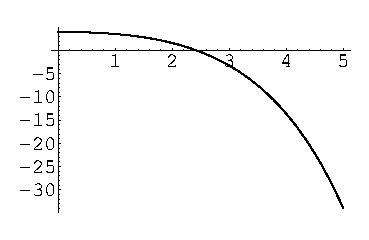
\includegraphics[width=0.3\textwidth]{ode/techniques_linear/6y5yy}
      \end{center}
      \caption{The solution decreases without bound at \textit{t} increases.}
      \label{figure 6y5yy}
    \end{figure}
    %%
    %%
    %%
  \item 
    We consider the problem
    \[
    y'' - 2 y' + 5 y = 0,\quad y(\pi/ 2) = 0,\quad y'(\pi/ 2) = 2.
    \]
    We make the substitution $y = \e^{\lambda x}$ in the differential equation.
    \begin{gather*}
      \lambda^2 - 2 \lambda + 5 = 0 \\
      \lambda = 1 \pm \sqrt{ 1 - 5 } \\
      \lambda = \{ 1 + \imath 2, 1 - \imath 2 \} 
    \end{gather*}
    The general solution of the differential equation is
    \[
    y = c_1 \e^{t} \cos(2 t) + c_2 \e^{t} \sin(2 t).
    \]
    We apply the initial conditions to determine the constants.
    \begin{gather*}
      y(\pi / 2) = 0 \quad \Rightarrow \quad - c_1 \e^{\pi / 2} = 0 \quad \Rightarrow \quad c_1 = 0 \\
      y'(\pi / 2) = 2 \quad \Rightarrow \quad -2 c_2 \e^{\pi / 2} = 2 \quad \Rightarrow \quad c_2 = - \e^{-\pi / 2}
    \end{gather*}
    The solution subject to the initial conditions is
    \[
    \boxed{
      y = - \e^{t-\pi/2} \sin(2 t).
      }
    \]
    The solution is plotted in Figure~\ref{figure y2y5y}.  The solution oscillates
    with an amplitude that tends to $\infty$ as $t \to \infty$.
    \begin{figure}[tb!]
      \begin{center}
        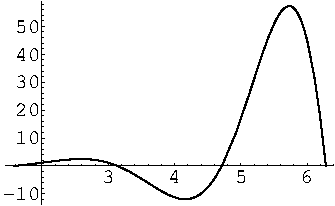
\includegraphics[width=0.3\textwidth]{ode/techniques_linear/y2y5y}
      \end{center}
      \caption{The amplitude of the oscilations increases without bound.}
      \label{figure y2y5y}
    \end{figure}
    %%
    %%
    %%
  \item 
    We consider the problem
    \[
    y'' + 4 y' + 4 y = 0,\quad y(-1) = 2,\quad y'(-1) = 1.
    \]
    We make the substitution $y = \e^{\lambda x}$ in the differential equation.
    \begin{gather*}
      \lambda^2 + 4 \lambda + 4 = 0 \\
      (\lambda + 2)^2 = 0 \\
      \lambda = -2
    \end{gather*}
    The general solution of the differential equation is
    \[
    y = c_1 \e^{-2 t} + c_2 t \e^{-2 t}.
    \]
    We apply the initial conditions to determine the constants.
    \begin{gather*}
      c_1 \e^{2} - c_2 \e^{2} = 2, \quad -2 c_1 \e^{2} + 3 c_2 \e^{2} = 1 \\
      c_1 = 7 \e^{-2}, \quad c_2 = 5 \e^{-2}
    \end{gather*}
    The solution subject to the initial conditions is
    \[
    \boxed{
      y = (7 + 5 t) \e^{-2 (t+1)} 
      }
    \]
    The solution is plotted in Figure~\ref{figure y4y4y}.  The solution vanishes
    as $t \to \infty$.
    \[
    \lim_{t \to \infty} (7 + 5 t) \e^{-2 (t+1)} 
    = \lim_{t \to \infty} \frac{7 + 5 t}{\e^{2 (t+1)}}
    = \lim_{t \to \infty} \frac{5}{2 \e^{2 (t+1)}}
    = 0
    \]
    \begin{figure}[tb!]
      \begin{center}
        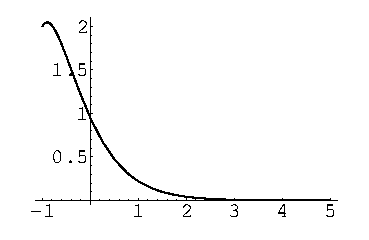
\includegraphics[width=0.3\textwidth]{ode/techniques_linear/y4y4y}
      \end{center}
      \caption{The solution vanishes as \textit{t} increases.}
      \label{figure y4y4y}
    \end{figure}
  \end{enumerate}
\end{Solution}











%% Find two linearly independent solutions to \[ y'' - 4 y' + 13 y = 0.   \]
\begin{Solution}
  \label{solution y-4y+13y}
  \[ 
  y'' - 4 y' + 13 y = 0. 
  \]
  With the substitution $y = \e^{\lambda x}$ we obtain
  \begin{gather*}
    \lambda^2 \e^{\lambda x} - 4 \lambda \e^{\lambda x} + 13 \e^{\lambda x} = 0 \\
    \lambda^2 - 4 \lambda + 13 = 0 \\
    \lambda = 2 \pm 3 i.
  \end{gather*}
  Thus two linearly independent solutions are
  \[ 
  \e^{(2 + 3i)x}, \quad \mathrm{and} \quad \e^{(2-3i)x}. 
  \]
  Noting that
  \begin{align*}
    \e^{(2+3i)x} &= \e^{2x} [\cos (3x) + \imath \sin(3x)] \\
    \e^{(2-3i)x} &= \e^{2x} [\cos (3x) - \imath \sin(3x)],
  \end{align*}
  we can write the two linearly independent solutions
  \[ 
  \boxed{ 
    y_1 = \e^{2x} \cos (3x), \qquad y_2 = \e^{2x} \sin(3x).
    } 
  \]
\end{Solution}






%% Find the general solution to \[ y''' - y'' + y' - y = 0. \]
\begin{Solution}
  \label{solution y-y+y-y=0}
  We note that 
  \[ 
  y''' - y'' + y' - y = 0 
  \]
  is a constant coefficient equation.  The substitution, $y = \e^{\lambda x}$,
  yields
  \begin{gather*}
    \lambda^3 - \lambda^2 + \lambda - 1 = 0 \\
    (\lambda-1)(\lambda-i)(\lambda+i) = 0.
  \end{gather*}
  The corresponding solutions are $\e^x$, $\e^{\imath x}$, and $\e^{-\imath x}$.  We 
  can write the general solution as
  \[ 
  \boxed{
    y = c_1 \e^x + c_2 \cos x + c_3 \sin x. 
    } 
  \]
\end{Solution}



%% Fundamental sets of solutions at $x = 0$ and $x = 1$.
\begin{Solution}
  \label{solution fund set x=0 x=1}
  We start with the equation $y'' + y = 0$.  We substitute $y = \e^{\lambda x}$
  into the differential equation to obtain
  \[
  \lambda^2 + 1 = 0, \qquad \lambda = \pm i.
  \]
  A linearly independent set of solutions is
  \[
  \{ \e^{\imath x}, \e^{-\imath x} \}.
  \]
  The 
  \hyperref[section The Fundamental Set of Solutions]
    {fundamental set of solutions}
  has the form
  \begin{align*}
    y_1 &= c_1 \e^{\imath x} + c_2 \e^{-\imath x}, \\
    y_2 &= c_3 \e^{\imath x} + c_4 \e^{-\imath x}.
  \end{align*}
  By applying the constraints
  \begin{alignat*}{2}
    y_1(0) &= 1, &\quad y_1'(0) &= 0, \\
    y_2(0) &= 0, &\quad y_2'(0) &= 1, 
  \end{alignat*}
  we obtain
  \begin{align*}
    y_1 &= \frac{\e^{\imath x} + \e^{-\imath x}}{2} = \cos x, \\
    y_2 &= \frac{\e^{\imath x} + \e^{-\imath x}}{\imath 2} = \sin x.
  \end{align*}

  Now consider the equation $y'' - y = 0$.  By substituting $y = \e^{\lambda x}$
  we find that a set of solutions is
  \[
  \{ \e^x, \e^{-x} \}.
  \]
  By taking linear combinations of these we see that another set of solutions 
  is
  \[
  \{ \cosh x, \sinh x \}.
  \]
  Note that this is the 
  \hyperref[section The Fundamental Set of Solutions]
    {fundamental set of solutions}.

  Next consider $y'' = 0$.  We can find the solutions by substituting
  $y = \e^{\lambda x}$ or by integrating the equation twice.  The 
  \hyperref[section The Fundamental Set of Solutions]
    {fundamental set of solutions}
  as $x = 0$ is
  \[
  \{ 1, x \}.
  \]

  Note that if $u(x)$ is a solution of a constant coefficient differential 
  equation, then $u(x+c)$ is also a solution.  Also note that if $u(x)$ 
  satisfies $y(0) = a$, $y'(0) = b$, then $u(x-x_0)$ satisfies 
  $y(x_0) = a$, $y'(x_0) = b$.  Thus the 
  \hyperref[section The Fundamental Set of Solutions]
    {fundamental sets of solutions}
  at $x = 1$ are
  \begin{enumerate}
  \item $\{ \cos(x-1), \sin(x-1) \}$,
  \item $\{ \cosh(x-1), \sinh(x-1) \}$,
  \item $\{ 1, x-1 \}$.
  \end{enumerate}
\end{Solution}







%% Damped harmonic motion
\begin{Solution}
  \label{solution damped harmonic motion}
  Let $y(t)$ denote the displacement of the mass from equilibrium.  
  The forces on the mass are $-k y(t)$ due to the spring and $- \mu y'(t)$
  due to friction.  We equate the external forces to $m y''(t)$ to find the
  differential equation of the motion.
  \begin{gather*}
    m y'' = - k y - \mu y' \\
    \boxed{
      y'' + \frac{\mu}{m} y' + \frac{k}{m} y = 0
      }
  \end{gather*}
  The solution which satisfies the initial conditions $y(0) = 0$, $y'(0) = 1$ is
  \[
  \boxed{
    y(t) = 
    \begin{cases}
      \e^{-\mu t / (2 m)} \frac{2 m}{\sqrt{\mu^2- 4 k m}} 
      \sinh \left( \sqrt{\mu^2 - 4 k m}\, t / (2 m) \right)
      \quad &\mathrm{if}\ \mu^2 > k m, \\
      \e^{-\mu t / (2 m)} \frac{2 m}{\sqrt{4 k m - \mu^2}} 
      \sin \left( \sqrt{4 k m - \mu^2}\, t / (2 m) \right)
      \quad &\mathrm{if}\ \mu^2 < k m, \\
      t \e^{-\mu t / (2 m)} 
      \quad &\mathrm{if}\ \mu^2 = k m.
    \end{cases}
    }
  \]
  We respectively call these cases: strongly damped, weakly damped and 
  critically damped.  In the case that $m = k = 1$ the solution is
  \[
  y(t) = 
  \begin{cases}
    \e^{-\mu t / 2} \frac{2}{\sqrt{\mu^2-4}} 
    \sinh \left( \sqrt{\mu^2 - 4}\, t / 2 \right)
    \quad &\mathrm{if}\ \mu > 2, \\
    \e^{-\mu t / 2} \frac{2}{\sqrt{4 - \mu^2}} 
    \sin \left( \sqrt{4 - \mu^2}\, t / 2 \right)
    \quad &\mathrm{if}\ \mu < 2, \\
    t \e^{- t} 
    \quad &\mathrm{if}\ \mu = 2.
  \end{cases}
  \]
  Note that when $t$ is large, $t \e^{-t}$ is much smaller than 
  $\e^{-\mu t / 2}$ for $\mu < 2$.  To prove this we examine the ratio of these
  functions as $t \to \infty$.
  \begin{align*}
    \lim_{t \to \infty} \frac{t \e^{-t}}{\e^{-\mu t / 2}}
    &= \lim_{t \to \infty} \frac{t}{\e^{(1 - \mu / 2) t}} \\
    &= \lim_{t \to \infty} \frac{1}{(1 - \mu / 2) \e^{(1 - \mu) t}} \\
    &= 0
  \end{align*}
  Using this result, we see that the critically damped solution decays faster
  than the weakly damped solution.  

  We can write the strongly damped solution as
  \[
  \e^{-\mu t / 2} \frac{2}{\sqrt{\mu^2-4}} 
  \left( \e^{\sqrt{\mu^2 - 4}\, t / 2} 
    - \e^{-\sqrt{\mu^2 - 4}\, t / 2} \right).
  \]
  For large $t$, the dominant factor is 
  $\e^{\left( \sqrt{\mu^2 - 4} - \mu \right) t / 2}$.  Note that for $\mu > 2$,
  \[
  \sqrt{\mu^2 - 4} = \sqrt{(\mu+2)(\mu-2)} > \mu - 2.
  \]
  Therefore we have the bounds
  \[
  -2 < \sqrt{\mu^2 - 4} - \mu < 0.
  \]
  This shows that the critically damped solution decays faster than the
  strongly damped solution.  $\mu = 2$ gives the fastest decaying solution.
  Figure~\ref{damped} shows the solution for $\mu = 4$, $\mu = 1$ and 
  $\mu = 2$.
  \begin{figure}[tb!]
    \begin{center}
      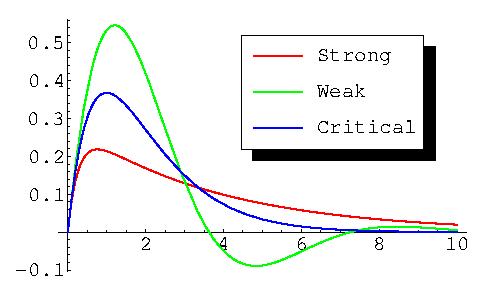
\includegraphics[width=0.4\textwidth]{ode/techniques_linear/damped}
    \end{center}
    \caption{Strongly, weakly and critically damped solutions.}
    \label{damped}
  \end{figure}
\end{Solution}
%% CONTINUE : Check the graph.










%% Show that $y = c \cos(x - \phi)$ is the general solution of 
\begin{Solution}
  \label{solution y=c cos x-phi}
  Clearly $y = c \cos(x - \phi)$ satisfies the differential equation 
  $y'' + y = 0$.  Since it is a two-parameter family of functions, 
  it must be the general solution.

  Using a trigonometric identity we can rewrite the solution as
  \[
  y = c \cos \phi \cos x + c \sin \phi \sin x.
  \]
  Setting this equal to $\sin x$ gives us the two equations
  \begin{align*}
    c \cos \phi &= 0, \\
    c \sin \phi &= 1,
  \end{align*}
  which has the solutions $c = 1$, $\phi = (2 n + 1/2) \pi$, and 
  $c = -1$, $\phi = (2 n - 1/2) \pi$, for $n \in \mathbb{Z}$.

  Clearly $y = c \cosh(x - \phi)$ satisfies the differential equation 
  $y'' - y = 0$.  Since it is a two-parameter family of functions, 
  it must be the general solution.

  Using a trigonometric identity we can rewrite the solution as
  \[
  y = c \cosh \phi \cosh x + c \sinh \phi \sinh x.
  \]
  Setting this equal to $\sinh x$ gives us the two equations
  \begin{align*}
    c \cosh \phi &= 0, \\
    c \sinh \phi &= 1,
  \end{align*}
  which has the solutions $c = -i$, $\phi = \imath (2 n + 1/2) \pi$, and 
  $c = i$, $\phi = \imath (2 n - 1/2) \pi$, for $n \in \mathbb{Z}$.
\end{Solution}







%% \frac{\dd^2 y}{\dd t^2} + 5 \frac{\dd y}{\dd t} + 6 y = 0
\begin{Solution}
  \label{solution y+5y+6y}
  We substitute $y = \e^{\lambda t}$ into the differential equation.
  \begin{gather*}
    \lambda^2 \e^{\lambda t} + 5 \lambda \e^{\lambda t} + 6 \e^{\lambda t} = 0 \\
    \lambda^2 + 5 \lambda + 6 = 0 \\
    (\lambda + 2)(\lambda + 3) = 0
  \end{gather*}
  The general solution of the differential equation is 
  \[
  y = c_1 \e^{-2 t} + c_2 \e^{-3 t}.
  \]
  The initial conditions give us the constraints:
  \begin{gather*}
    c_1 + c_2 = 1, \\
    -2 c_1 - 3 c_2 = V.
  \end{gather*}
  The solution subject to the initial conditions is
  \[
  \boxed{
    y = (3 + V) \e^{-2 t} - (2 + V) \e^{-3 t}.
    }
  \]
  This solution will be non-negative for $t > 0$ if $V \geq -3$.
\end{Solution}






%% y'' + \sign(x) y = 0, \quad -\infty < x < \infty.
\begin{Solution}
  \label{solution y+sign y}
  For negative $x$, the differential equation is
  \[
  y'' - y = 0.
  \]
  We substitute $y = \e^{\lambda x}$ into the differential equation to find
  the solutions.
  \begin{gather*}
    \lambda^2 - 1 = 0 \\
    \lambda = \pm 1 \\
    y = \left\{ \e^x, \e^{-x} \right\} \\
    \intertext{We can take linear combinations to write the solutions in terms of
      the hyperbolic sine and cosine.}
    y = \left\{ \cosh(x), \sinh(x) \right\}
  \end{gather*}

  For positive $x$, the differential equation is
  \[
  y'' + y = 0.
  \]
  We substitute $y = \e^{\lambda x}$ into the differential equation to find
  the solutions.
  \begin{gather*}
    \lambda^2 + 1 = 0 \\
    \lambda = \pm \imath \\
    y = \left\{ \e^{\imath x}, \e^{-\imath x} \right\} \\
    \intertext{We can take linear combinations to write the solutions in terms of
      the sine and cosine.}
    y = \left\{ \cos(x), \sin(x) \right\}
  \end{gather*}

  We will find the 
  \hyperref[section The Fundamental Set of Solutions]
    {fundamental set of solutions}
  at $x = 0$.  That is, we will
  find a set of solutions, $\{y_1, y_2\}$ that satisfy the conditions:
  \begin{alignat*}{2}
    y_1(0) &= 1 &\quad y_1'(0) &= 0 \\
    y_2(0) &= 0 &\quad y_2'(0) &= 1 \\
  \end{alignat*}
  Clearly, these solutions are
  \[
  \boxed{
    y_1 = \begin{cases}
      \cosh(x) &x < 0 \\
      \cos(x) &x \geq 0
    \end{cases}
    \qquad
    y_2 = \begin{cases}
      \sinh(x) &x < 0 \\
      \sin(x) &x \geq 0
    \end{cases}
    }
  \]
\end{Solution}








%%-----------------------------------------------------------------------------
\begin{large}
  \noindent
  \textbf{Euler Equations}
\end{large}








%% x^2 y'' + x y' + y = 0, \qquad x > 0.
\begin{Solution}
  \label{solution x2y+xy+y}
  We consider an Euler equation,
  \[
  x^2 y'' + x y' + y = 0, \quad x > 0.
  \]
  We make the change of independent variable $\xi = \ln x$, $u(\xi) = y(x)$
  to obtain
  \[
  u'' + u = 0.
  \]
  We make the substitution $u(\xi) = \e^{\lambda \xi}$.
  \begin{gather*}
    \lambda^2 + 1 = 0 \\
    \lambda = \pm i
  \end{gather*}
  A set of linearly independent solutions for $u(\xi)$ is
  \[
  \{ \e^{\imath \xi}, \e^{-\imath \xi} \}.
  \]
  Since
  \[
  \cos \xi = \frac{\e^{\imath \xi} + \e^{-\imath \xi} }{2} \quad \mathrm{and} \quad
  \sin \xi = \frac{\e^{\imath \xi} - \e^{-\imath \xi} }{\imath 2},
  \]
  another linearly independent set of solutions is
  \[
  \{ \cos \xi, \sin \xi \}.
  \]
  The general solution for $y(x)$ is
  \[
  \boxed{
    y(x) = c_1 \cos( \ln x ) + c_2 \sin( \ln x ).
    }
  \]
\end{Solution}





%% Find the general solution of \[ x^2 y'' - 2 x y + 2 y = 0.  \]
\begin{Solution}
  \label{solution x2y-2xy+2y}
  Consider the differential equation
  \[ 
  x^2 y'' - 2 x y + 2 y = 0. 
  \]
  With the substitution $y = x^{\lambda}$ this equation becomes
  \begin{gather*}
    \lambda(\lambda-1) - 2 \lambda + 2 = 0 \\
    \lambda^2 - 3 \lambda + 2 = 0 \\
    \lambda = 1, 2.
  \end{gather*}
  The general solution is then
  \[ 
  \boxed{ y = c_1 x + c_2 x^2.} 
  \]
\end{Solution}



%% Find the general solution of \[ x y''' + y'' + \frac{1}{x} y' = 0. \]
\begin{Solution}
  \label{solution xy+y+1xy}
  We note that
  \[ 
  x y''' + y'' + \frac{1}{x} y' = 0 
  \]
  is an Euler equation.  The substitution $y = x^\lambda$ yields
  \begin{gather*}
    \lambda^3 - 3 \lambda^2 + 2 \lambda + \lambda^2 - \lambda + \lambda = 0 \\
    \lambda^3 - 2 \lambda^2 + 2 \lambda = 0.
  \end{gather*}
  The three roots of this algebraic equation are
  \begin{alignat*}{3}
    \lambda &= 0,   &\quad   \lambda &= 1 + i,       &\quad  \lambda &= 1 - \imath \\
    \intertext{The corresponding solutions to the differential equation are}
    y &= x^0        &\quad  y &= x^{1 + \imath}    &\quad  y &= x^{1 - \imath} \\
    y &= 1          &\quad  y &= x \e^{\imath \ln x}      &\quad  y &= x \e^{-\imath \ln x}.
  \end{alignat*}
  We can write the general solution as
  \[ 
  \boxed{ 
    y = c_1 + c_2 x \cos(\ln x) + c_3 \sin(\ln x). 
    } 
  \]
\end{Solution}






%% Find the general solution of \[ x^2 y'' + (2 a + 1) x y' + b y = 0.
\begin{Solution}
  \label{solution x2y+2a1xy+by}
  We substitute $y = x^\lambda$ into the differential equation.
  \begin{gather*}
    x^2 y'' + (2 a + 1) x y' + b y = 0 \\
    \lambda(\lambda - 1) + (2 a + 1) \lambda + b = 0 \\
    \lambda^2 + 2 a \lambda + b  = 0 \\
    \lambda = -a \pm \sqrt{a^2 - b}
  \end{gather*}
  For $a^2 > b$ then the general solution is
  \[
  y = c_1 x^{-a + \sqrt{a^2 - b}} + c_2 x^{-a - \sqrt{a^2 - b}}.
  \]
  For $a^2 < b$, then the general solution is
  \[
  y = c_1 x^{-a + \imath \sqrt{b - a^2}} + c_2 x^{-a - \imath \sqrt{b - a^2}}.
  \]
  By taking the sum and difference of these solutions, we can write the 
  general solution as
  \[
  y = c_1 x^{-a} \cos \left( \sqrt{b - a^2}\, \ln x \right)
  + c_2 x^{-a} \sin \left( \sqrt{b - a^2}\, \ln x \right).
  \]
  For $a^2 = b$, the quadratic in lambda has a double root at $\lambda = a$.
  The general solution of the differential equation is
  \[
  y = c_1 x^{-a} + c_2 x^{-a} \ln x.
  \]
  In summary, the general solution is:
  \[
  \boxed{
    y = 
    \begin{cases}
      x^{-a} \left( c_1 x^{\sqrt{a^2 - b}} 
        + c_2 x^{- \sqrt{a^2 - b}} \right)
      \quad &\mathrm{if}\ a^2 > b, \\
      x^{-a} \left( c_1 \cos \left( \sqrt{b - a^2}\, \ln x \right)  
        + c_2 \sin \left( \sqrt{b - a^2}\, \ln x \right) \right)
      \quad &\mathrm{if}\ a^2 < b, \\
      x^{-a} \left( c_1 + c_2 \ln x \right)
      \quad &\mathrm{if}\ a^2 = b. 
    \end{cases}
    }
  \]
\end{Solution}





%% Solution defined for all values of the parameter.
\begin{Solution}
  \label{solution y1=eax}
  For $a \neq 0$, two linearly independent solutions of
  \[
  y'' - a^2 y = 0
  \]
  are 
  \[
  y_1 = \e^{a x}, \quad y_2 = \e^{-a x}.
  \]
  For $a = 0$, we have
  \[
  y_1 = \e^{0 x} = 1, \quad y_2 = x \e^{0 x} = x.
  \]
  In this case the solution are defined by
  \[
  y_1 = \left[\e^{a x} \right]_{a = 0}, \quad
  y_2 = \left[\frac{\dd}{\dd a} \e^{a x} \right]_{a = 0}.
  \]
  By the definition of differentiation, $f'(0)$ is 
  \[
  f'(0) = \lim_{a \to 0} \frac{f(a) - f(-a)}{2a}.
  \]
  Thus the second solution in the case $a = 0$ is
  \[
  y_2 = \lim_{a \to 0} \frac{\e^{a x} - \e^{-a x}}{a}
  \]
  Consider the solutions
  \[
  y_1 = \e^{a x}, \quad
  y_2 = \lim_{\alpha \to a} \frac{\e^{\alpha x} - \e^{-\alpha x}}{\alpha}.
  \]
  Clearly $y_1$ is a solution for all $a$.  For $a \neq 0$, $y_2$ is a linear
  combination of $\e^{a x}$ and $\e^{-a x}$ and is thus a solution.  
  Since the coefficient of $\e^{-a x}$ in this linear combination is non-zero,
  it is linearly independent to $y_1$.  For $a = 0$, $y_2$ is one half
  the derivative of $\e^{a x}$ evaluated at $a = 0$.  Thus it is a solution.


  For $a \neq 0$, two linearly independent solutions of
  \[
  x^2 y'' + x y' - a^2 y = 0
  \]
  are 
  \[
  y_1 = x^a, \quad y_2 = x^{-a}.
  \]
  For $a = 0$, we have
  \[
  y_1 = \left[ x^a \right]_{a = 0} = 1, \quad 
  y_2 = \left[ \frac{\dd}{\dd a} x^a \right]_{a = 0} = \ln x.
  \]
  Consider the solutions
  \[
  y_1 = x^a, \quad
  y_2 = \frac{x^a - x^{-a}}{a}
  \]
  Clearly $y_1$ is a solution for all $a$.  For $a \neq 0$, $y_2$ is a linear
  combination of $x^a$ and $x^{-a}$ and is thus a solution.  
  For $a = 0$, $y_2$ is one half the derivative of $x^a$ evaluated at $a = 0$.  
  Thus it is a solution.
\end{Solution}








%% Find two linearly independent solutions (i.e., the general solution) of 
\begin{Solution}
  \label{solution x2y-2xy+2y=0}
  \begin{enumerate}
    %%
    %%
    %%
  \item
    \[
    x^2 y'' - 2 x y' + 2 y = 0
    \]
    We substitute $y = x^\lambda$ into the differential equation.
    \begin{gather*}
      \lambda (\lambda - 1) - 2 \lambda + 2 = 0 \\
      \lambda^2 - 3 \lambda + 2 = 0 \\
      (\lambda - 1)(\lambda - 2) = 0 \\
      \boxed{
        y = c_1 x + c_2 x^2
        }
    \end{gather*}
    %%
    %%
    %%
  \item
    \[
    x^2 y'' - 2 y = 0
    \]
    We substitute $y = x^\lambda$ into the differential equation.
    \begin{gather*}
      \lambda (\lambda - 1) - 2 = 0 \\
      \lambda^2 - \lambda - 2 = 0 \\
      (\lambda + 1)(\lambda - 2) = 0 \\
      \boxed{
        y = \frac{c_1}{x} + c_2 x^2
        }
    \end{gather*}
    %%
    %%
    %%
  \item
    \[
    x^2 y'' - x y' + y = 0
    \]
    We substitute $y = x^\lambda$ into the differential equation.
    \begin{gather*}
      \lambda (\lambda - 1) - \lambda + 1 = 0 \\
      \lambda^2 - 2 \lambda + 1 = 0 \\
      (\lambda - 1)^2 = 0 \\
      \intertext{Since there is a double root, the solution is:}
      \boxed{
        y = c_1 x + c_2 x \ln x.
        }
    \end{gather*}
  \end{enumerate}
\end{Solution}







%%-----------------------------------------------------------------------------
\begin{large}
  \noindent
  \textbf{Exact Equations}
\end{large}



%% Solve the differential equation \[ y'' + y' \sin x + y \cos x  = 0. \]
\begin{Solution}
  \label{solution y+ysinx+ycosx}
  We note that
  \[ 
  y'' + y' \sin x + y \cos x = 0 
  \]
  is an exact equation.
  \begin{gather*}
    \frac{\dd}{\dd x} [ y' + y \sin x] = 0 \\
    y' + y \sin x = c_1 \\
    \frac{\dd}{\dd x} \left[ y \e^{-\cos x} \right] = c_1 \e^{-\cos x} \\
    \boxed{ 
      y = c_1 \e^{\cos x} \int \e^{-\cos x}\,\dd x + c_2 \e^{\cos x} 
      }
  \end{gather*}
\end{Solution}



%%-----------------------------------------------------------------------------
\begin{large}
  \noindent
  \textbf{Equations Without Explicit Dependence on \protect$ \mathbf{y} \protect$}
\end{large}

%%-----------------------------------------------------------------------------
\begin{large}
  \noindent
  \textbf{Reduction of Order}
\end{large}





%% (1-x^2) y'' - 2 x y' + 2 y = 0, \quad -1 < x < 1
\begin{Solution}
  \label{solution 1-x2y-2xy+2y}
  \[
  (1-x^2) y'' - 2 x y' + 2 y = 0, \quad -1 < x < 1
  \]
  We substitute $y = x$ into the differential equation to check that it is
  a solution.
  \[
  (1-x^2) (0) - 2 x (1) + 2 x = 0
  \]
  We look for a second solution of the form $y = x u$.  We substitute 
  this into the differential equation and use the fact that $x$ is a solution.
  \begin{gather*}
    (1-x^2) (x u'' + 2 u') - 2 x (x u' + u) + 2 x u = 0 \\
    (1-x^2) (x u'' + 2 u') - 2 x (x u') = 0 \\
    (1-x^2) x u'' + (2 - 4 x^2) u' = 0 \\
    \frac{u''}{u'} = \frac{2 - 4 x^2}{x(x^2 - 1)} \\
    \frac{u''}{u'} = - \frac{2}{x} + \frac{1}{1-x} - \frac{1}{1+x} \\
    \ln(u') = -2 \ln(x) - \ln(1-x) - \ln(1+x) + \mathrm{const} \\
    \ln(u') = \ln \left( \frac{c}{x^2 (1-x)(1+x)} \right) \\
    u' = \frac{c}{x^2 (1-x)(1+x)} \\
    u' = c \left( \frac{1}{x^2} + \frac{1}{2(1-x)} + \frac{1}{2(1+x)} \right) \\
    u = c \left( - \frac{1}{x} - \frac{1}{2} \ln(1-x) + \frac{1}{2} \ln(1+x) 
    \right) + \mathrm{const} \\
    u = c \left( - \frac{1}{x} + \frac{1}{2} \ln \left( \frac{1+x}{1-x} \right)
    \right)
    + \mathrm{const} 
  \end{gather*}
  A second linearly independent solution is
  \[
  \boxed{
    y = - 1 + \frac{x}{2} \ln \left( \frac{1+x}{1-x} \right).
    }
  \]
\end{Solution}







%% Reduction of order where $\e^x$ is one solution.
\begin{Solution}
  \label{solution y-x+1xy+1xy}
  We are given that $y = \e^x$ is a solution of
  \[ 
  y'' - \frac{x + 1}{x} y' + \frac{1}{x} y = 0.
  \]
  To find another linearly independent solution, we will use reduction of 
  order.  Substituting 
  \begin{align*}
    y &= u \e^x \\ 
    y' &= (u' + u)\e^x \\
    y'' &= (u'' + 2u' + u)\e^x
  \end{align*}
  into the differential equation yields
  \begin{gather*}
    u'' + 2u' + u - \frac{x+1}{x} (u' + u) + \frac{1}{x} u = 0. \\
    u'' + \frac{x-1}{x} u' = 0 \\
    \frac{\dd}{\dd x} \left[ u' \exp\left(\int \left(1 - \frac{1}{x}\right)\,\dd x 
      \right) \right] = 0 \\
    u' \e^{x - \ln x} = c_1 \\
    u' = c_1 x \e^{-x} \\
    u = c_1 \int x \e^{-x}\,\dd x + c_2  \\
    u = c_1 (x \e^{-x} + \e^{-x}) + c_2  \\
    y = c_1 (x + 1) + c_2 \e^x  \\
    \intertext{Thus a second linearly independent solution is}
    \boxed{ 
      y = x+1. 
      }
  \end{gather*}
\end{Solution}













%% Reduction of order where $x$ is one solution.
\begin{Solution}
  \label{solution 1-2xy+4xy-4y}
  We are given that $y = x$ is a solution of
  \[ 
  (1 - 2 x) y'' + 4 x y' - 4 y = 0.
  \]
  To find another linearly independent solution, we will use reduction of 
  order.  Substituting 
  \begin{align*}
    y &= x u \\
    y' &= x u' + u \\
    y'' &= x u'' + 2 u'
  \end{align*}
  into the differential equation yields
  \begin{gather*}
    (1 - 2 x) (x u'' + 2 u') + 4 x (x u' + u) - 4 x u = 0, \\
    (1 - 2 x) x u'' + (4 x^2 - 4 x + 2) u' = 0, \\
    \frac{u''}{u'} = \frac{4 x^2 - 4 x + 2}{x (2 x - 1)}, \\
    \frac{u''}{u'} = 2 - \frac{2}{x} + \frac{2}{2 x - 1}, \\
    \ln(u') = 2 x - 2 \ln x + \ln(2 x - 1) + \mathrm{const}, \\
    u' = c_1 \left( \frac{2}{x} - \frac{1}{x^2} \right) \e^{2 x}, \\
    u = c_1 \frac{1}{x} \e^{2 x} + c_2, \\
    \boxed{
      y = c_1 \e^{2 x} + c_2 x.
      }
  \end{gather*}
\end{Solution}






\begin{Solution}
  \label{solution (x-1)y-xy+y=0}
  One solution of
  \[ 
  (x-1) y\prime\prime - x y\prime + y = 0, 
  \]
  is $y_1 = \e^x$.  We find a second solution with reduction of order.  We 
  make the substitution $y_2 = u \e^x$ in the differential equation.
  We determine $u$ up to an additive constant.
  \begin{gather*}
    (x - 1) (u'' + 2 u' + u) \e^x - x (u' + u) \e^x + u \e^x = 0
    \\
    (x - 1) u'' + (x - 2) u' = 0
    \\
    \frac{u''}{u'} = - \frac{x - 2}{x - 1} = -1 + \frac{1}{x - 1}
    \\
    \ln | u' | = - x + \ln |x-1| + c
    \\
    u' = c (x - 1) \e^{-x}
    \\
    u = -c x \e^{-x}
  \end{gather*}
  The second solution of the differential equation is $y_2 = x$.
\end{Solution}







%%-----------------------------------------------------------------------------
\begin{large}
  \noindent
  \textbf{*Reduction of Order and the Adjoint Equation}
\end{large}
















\raggedbottom
}









